\documentclass[11pt]{article}
\usepackage[margin=1in]{geometry}
\usepackage{graphicx}
\usepackage{amsmath,amssymb}
\usepackage{booktabs}
\usepackage{caption}
\usepackage{subcaption}
\usepackage{float}
\usepackage{array}
\usepackage{siunitx}
\usepackage[hidelinks]{hyperref}
\graphicspath{{./}{figs/}{figures/}{pub_figs/}{openfoam/doc_figs/}{openfoam/chamber42_3d/calibration/}}
\captionsetup{font=small,labelfont=bf}
\setlength{\parskip}{4pt}

\title{\textbf{A Three-Dimensional VOF Phase-Change Simulation Framework\\
for a Subcooled Pool-Boiling Chamber with a Submerged Tube-Bundle Condenser}}
\author{[Author list]\\
\small Thermal Analysis Laboratory, Department of Mechanical Engineering\\
\small Rochester Institute of Technology, Rochester, NY, USA}
\date{\today}

\begin{document}
\maketitle

\begin{abstract}
\noindent
This paper specifies a three-dimensional volume-of-fluid (VOF) phase-change simulation framework
for a closed, subcooled pool-boiling chamber with a partially submerged tube-bundle condenser,
built on the true CAD geometry of the apparatus. It documents a verified body-fitted mesh
(\num{299656} cells, passing \texttt{checkMesh}), the governing equations and numerical scheme
for the incompressible two-phase mixture with interface capturing, buoyancy, surface tension, and
a Lee phase-change closure, the condenser coolant-side flow routing, and the measured boiling
curves and thermal resistances that serve as validation targets. A calibration-to-validation
workflow is defined in which the phase-change coefficients are fit against a measured boiling
curve and critical heat flux and the converged solution is then compared point by point against
experiment. A reduced-cost two-dimensional demonstration establishes that the pipeline runs and
behaves physically while showing why quantitative calibration requires the resolved
three-dimensional mesh. Consistent with the project's integrity standard, the framework is
presented as a specification with verification references only: no unconverged or surrogate field
is reported as a phase-change result, and the calibration and overlay against experiment await the
converged production run.
\end{abstract}

\tableofcontents
\clearpage

\section{Overview and scope of the CFD framework}
The apparatus modeled here is the closed subcooled pool-boiling chamber with a partially
submerged tube-bundle condenser of Shukla and Kandlikar~\cite{shukla2024}, whose thermal
performance across two evaporator surfaces, two condenser bundles, and four coolant inlet
temperatures is characterized and predicted in a companion reduced-order study of the same
apparatus; the present work develops the complementary high-fidelity route, a three-dimensional
VOF simulation with phase change that resolves the boiling and condensation fields on the real
geometry.

This document specifies that framework completely and reproducibly, and it assembles
the experimental reference, coolant operating conditions, measured boiling curves, and
thermal resistances for both condensers, that the simulation is required to reproduce.
Following the integrity standard of the broader project, we keep a hard line between
three sources: measured data, the validated reduced-order model, and the CFD. The
boiling-curve and resistance comparisons in Section~\ref{of-sec:reference} are
\emph{experiment versus the reduced-order model}; they are the CFD's target, not CFD
output. The CFD field contours and the CFD-to-experiment overlay require the converged
run of Section~\ref{of-sec:post} and are not fabricated here.

\section{Apparatus geometry}
\label{of-sec:geom}
The full apparatus geometry, including both evaporator surfaces and both condenser bundles, is
documented in the companion reduced-order study; this section records only the geometric detail
needed to reproduce the CFD mesh.

\subsection{Chamber and computational domain}
The domain is the chamber interior, $80 \times 80 \times \SI{42}{mm}$ ($x$~width,
$y$~tube axis, $z$~height), gravity along $-z$ (Fig.~\ref{of-fig:domain}). The 42 condenser
tubes are imported as a triangulated surface at their measured CAD positions; the bundle
straddles the liquid level so the lower rows are submerged and the upper rows sit in the
vapor space. The heated chip ($34.5\times\SI{32}{mm}$, \SI{11.04}{cm^2} footprint) is
centered on the floor, and the pool fills the lower \SI{16.8}{mm} (about 40\%).
Figure~\ref{of-fig:geom} gives the dimensioned cross-section with the real staggered tube
layout.

\begin{figure}[H]
\centering
\begin{subfigure}{0.56\textwidth}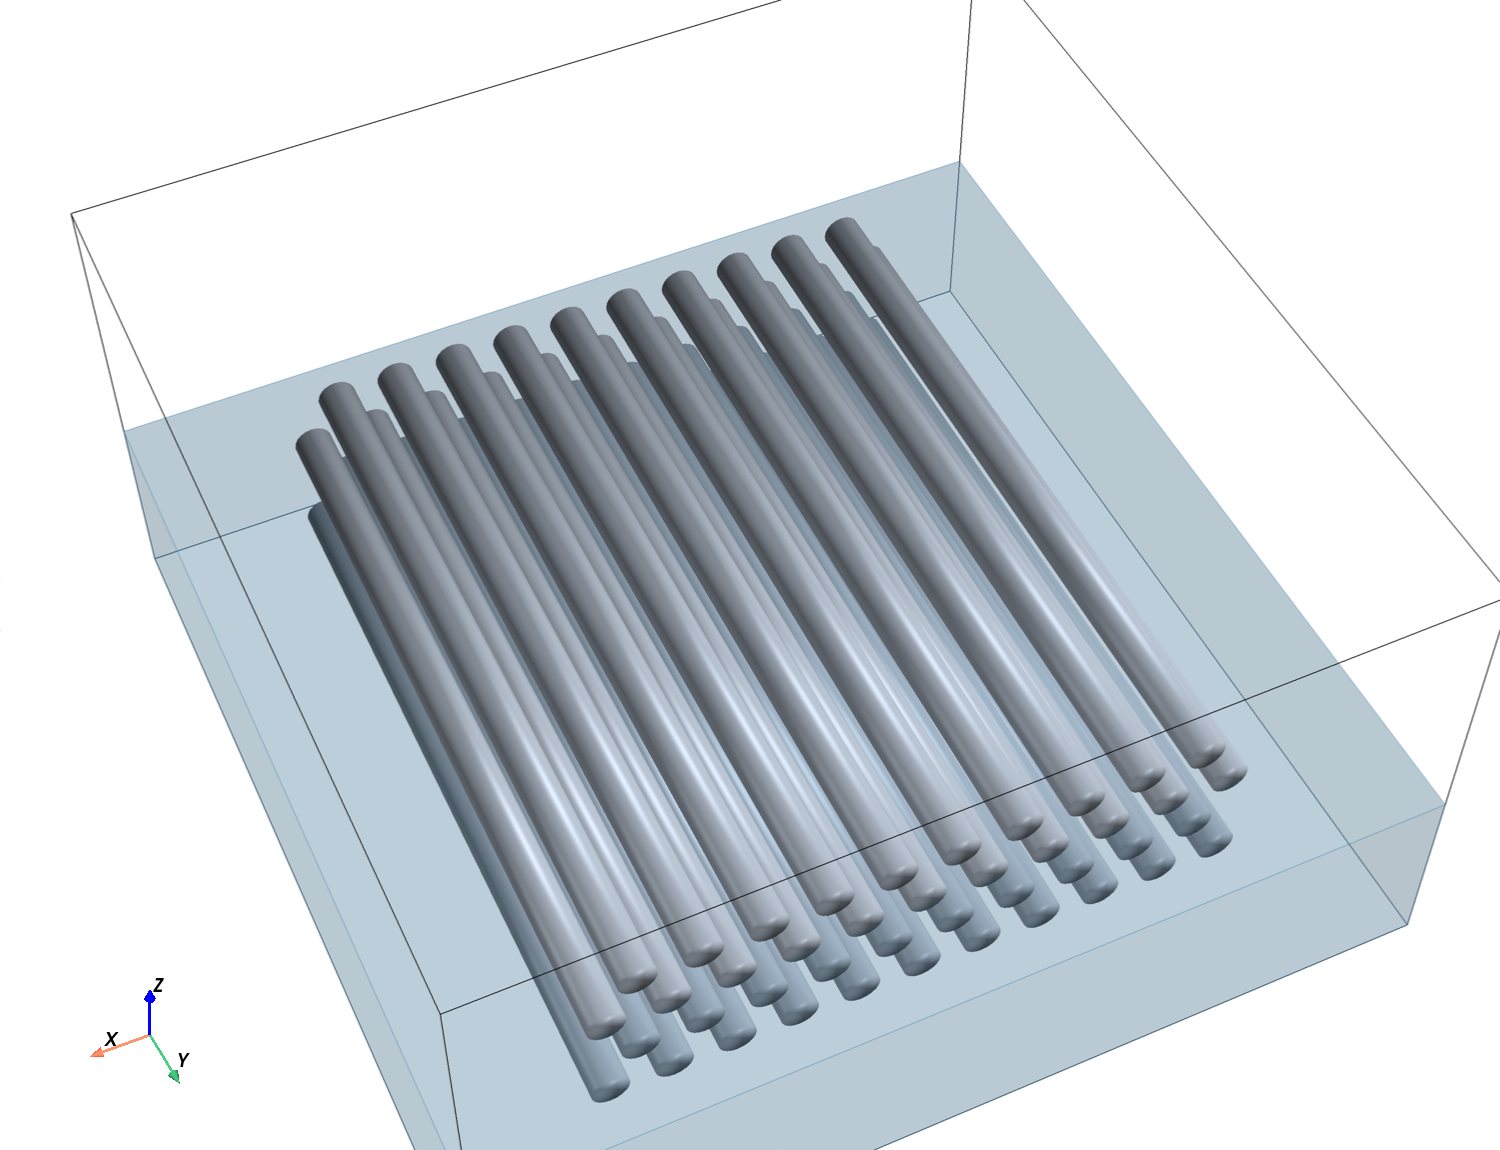
\includegraphics[width=\textwidth]{fig_domain.png}
\caption{Isometric.}\end{subfigure}\hfill
\begin{subfigure}{0.42\textwidth}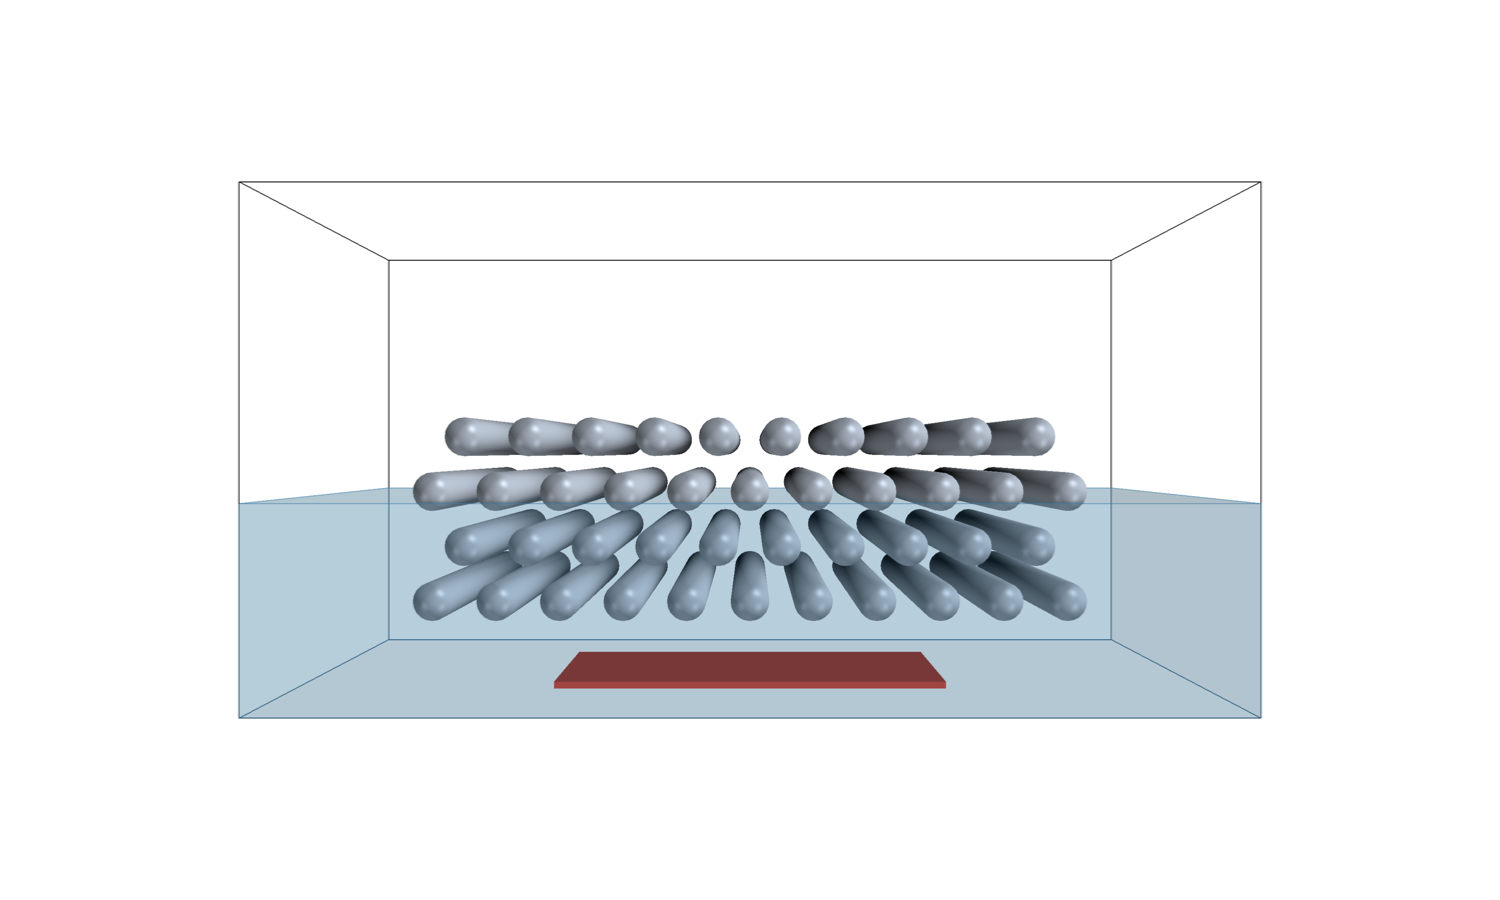
\includegraphics[width=\textwidth]{fig_domain_front.png}
\caption{Front ($x$--$z$).}\end{subfigure}
\caption{Computational domain: chamber (outline), 42-tube bundle (grey), heated chip
(red), subcooled pool (blue) at 40\% fill. The bundle straddles the interface.}
\label{of-fig:domain}
\end{figure}

\begin{figure}[H]
\centering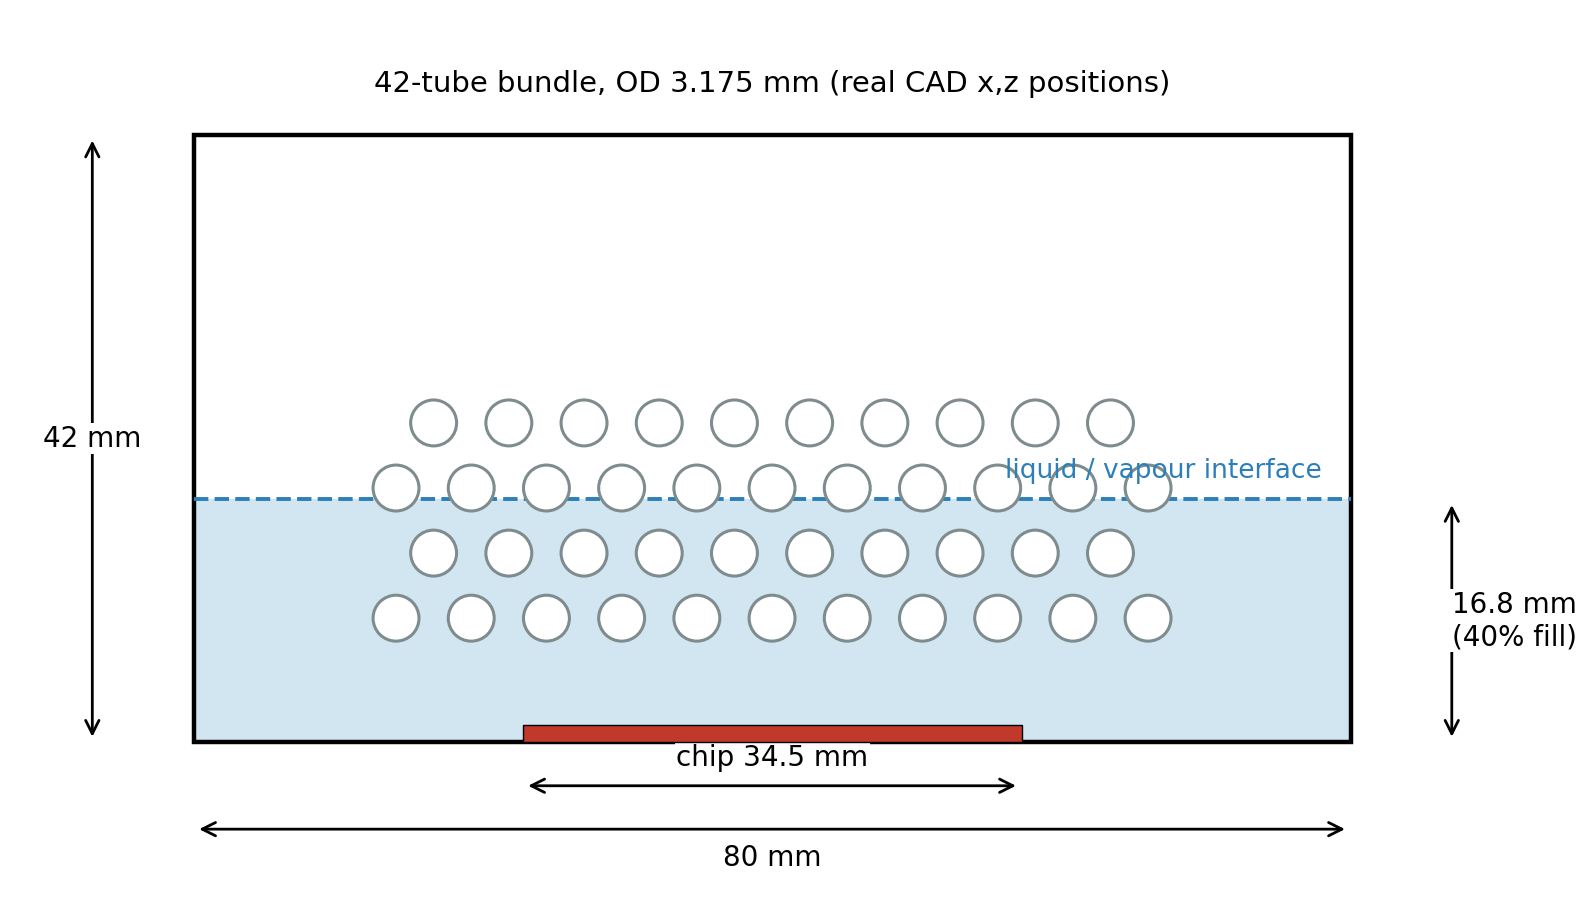
\includegraphics[width=0.80\textwidth]{fig_geom_dims.png}
\caption{Dimensioned $x$--$z$ cross-section with the measured 42-tube layout; the dashed
line is the initial interface at \SI{16.8}{mm}.}
\label{of-fig:geom}
\end{figure}

\subsection{Evaporator surfaces}
Both chips share the \SI{11.04}{cm^2} copper footprint; the plain chip is a smooth boiling
surface and the enhanced chip carries the open Cooke--Kandlikar microchannels detailed in the
companion reduced-order study (Fig.~\ref{of-fig:micro}). In the CFD the plain surface is modeled
as a flat heated wall; resolving or sub-grid-modeling the microchannel surface is a planned
extension (Section~\ref{of-sec:next}).

\begin{figure}[H]
\centering
\begin{subfigure}{0.50\textwidth}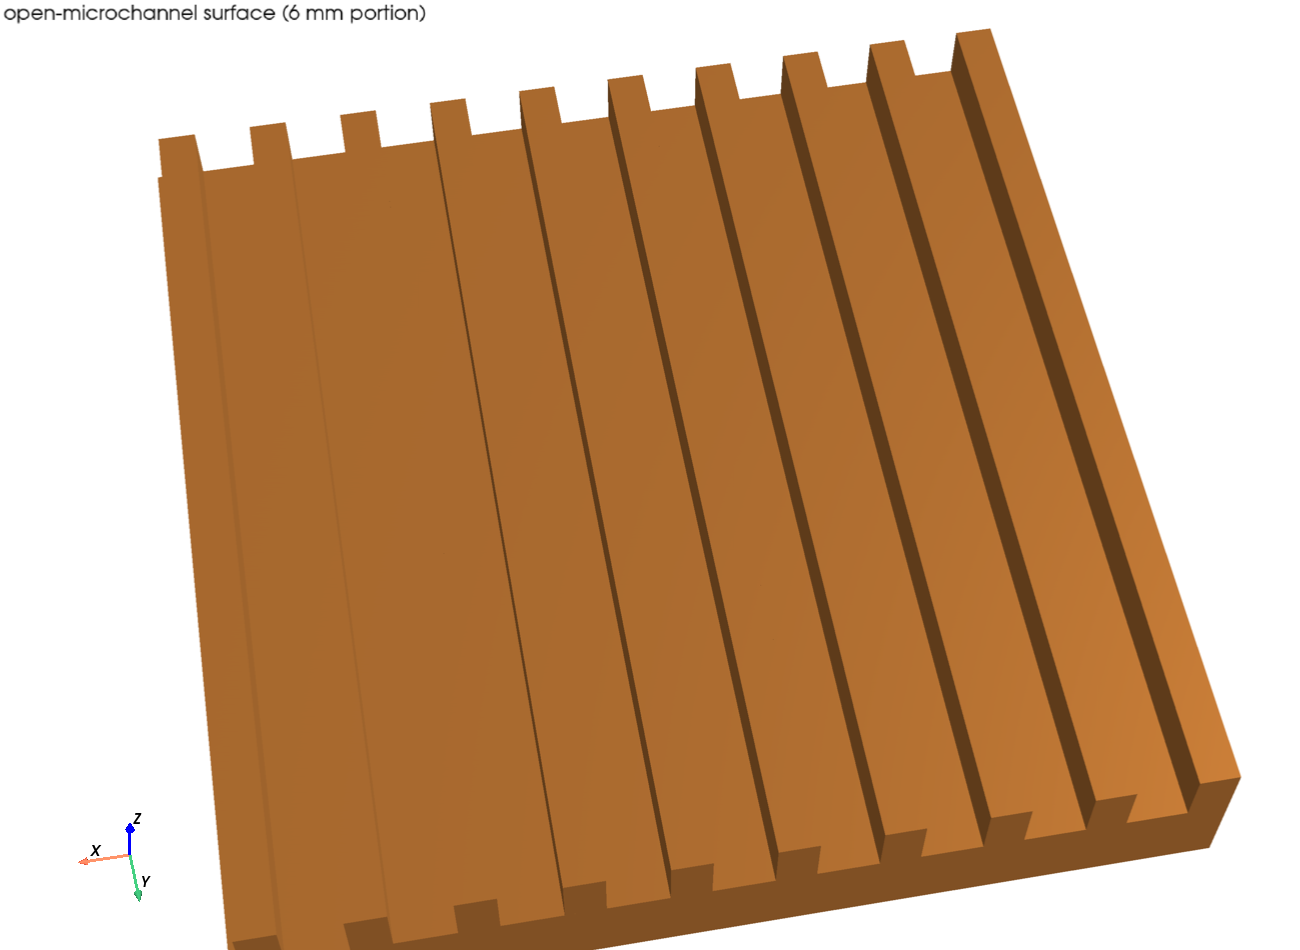
\includegraphics[width=\textwidth]{fig_micro_3d.png}
\caption{Surface portion (6\,mm).}\end{subfigure}\hfill
\begin{subfigure}{0.48\textwidth}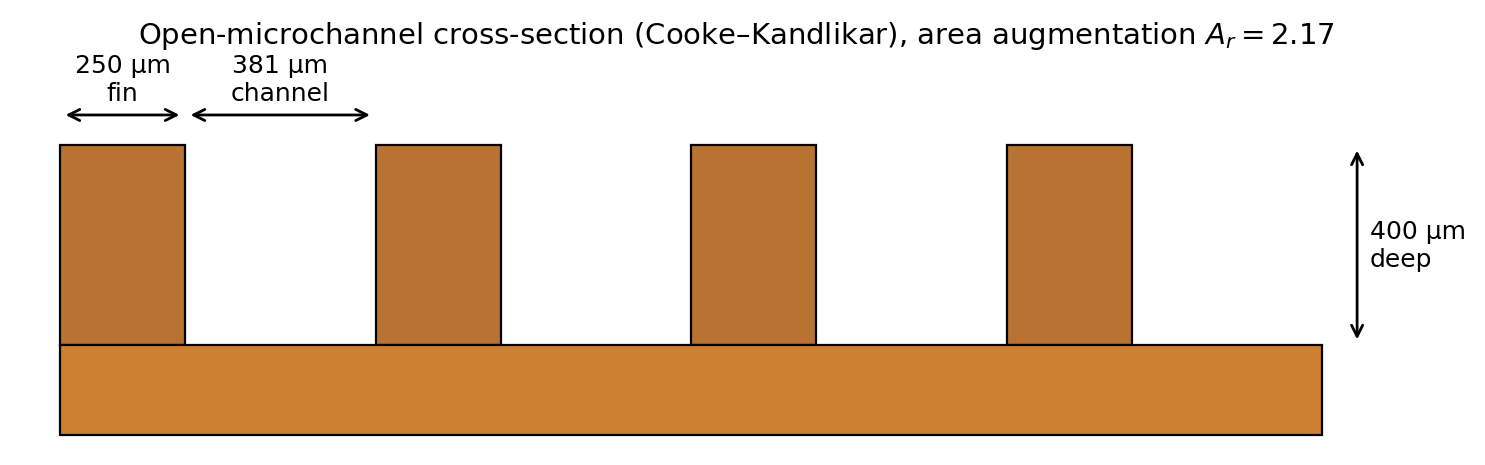
\includegraphics[width=\textwidth]{fig_micro_section.png}
\caption{Cross-section with dimensions.}\end{subfigure}
\caption{Open-microchannel evaporator surface (Cooke--Kandlikar geometry).}
\label{of-fig:micro}
\end{figure}

\subsection{Condenser bundles}
Two bundles are studied (Fig.~\ref{of-fig:cond}, Table~\ref{of-tab:cond}). The 33-tube bundle
uses fewer, larger tubes (OD \SI{4.76}{mm}) with open manifolds; the 42-tube bundle uses
more, smaller tubes (OD \SI{3.175}{mm}) in a confined in-chamber manifold. The CFD case
documented here is the 42-tube geometry; a 33-tube case is a separate build
(Section~\ref{of-sec:next}).

\begin{figure}[H]
\centering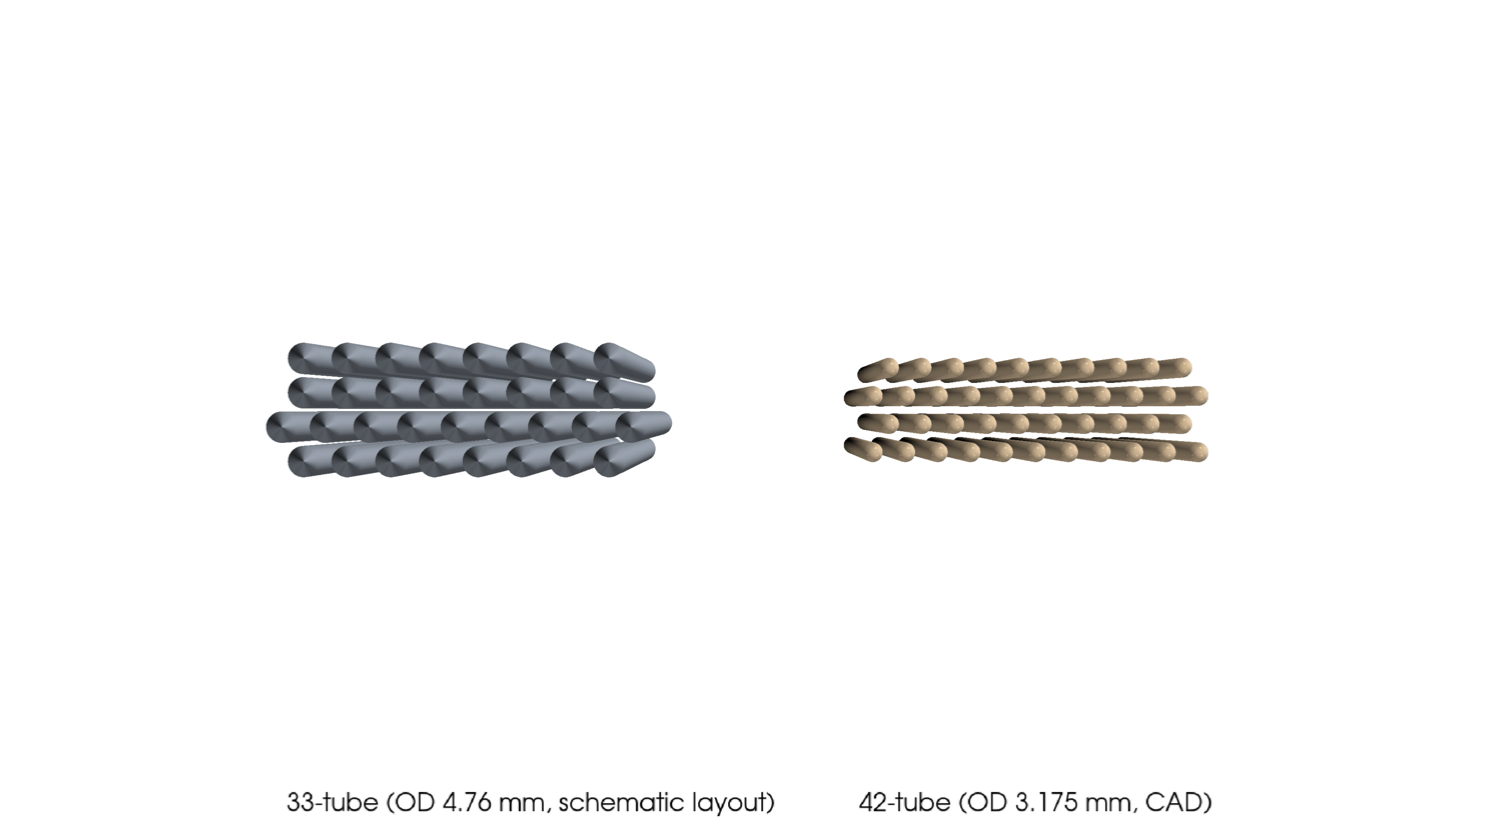
\includegraphics[width=0.92\textwidth]{fig_condensers.png}
\caption{The two condenser bundles to scale: 33-tube (OD \SI{4.76}{mm}; layout
schematic, CAD positions not available) and 42-tube (OD \SI{3.175}{mm}, from CAD).}
\label{of-fig:cond}
\end{figure}

\begin{table}[H]
\centering\caption{Condenser bundle geometry.}\label{of-tab:cond}
\begin{tabular}{lccccc}
\toprule
Bundle & Tubes & OD (mm) & ID (mm) & $L$ (mm) & Layout\\
\midrule
33-tube & 33 & 4.76 & 3.14 & 95.0 & open manifold\\
42-tube & 42 & 3.175 & 1.39 & 62.6 & confined\\
\bottomrule
\end{tabular}
\end{table}

\section{Governing equations}
\label{of-sec:equations}
The solver \texttt{interCondensatingEvaporatingFoam}, part of the OpenFOAM finite-volume
framework~\cite{of-weller1998}, advances a single incompressible two-phase (water/vapor) mixture
with volume-of-fluid interface capturing~\cite{of-hirt1981}, buoyancy,
surface tension, and a volumetric phase-change source. The flow is treated as laminar
(justified in Section~\ref{of-sec:dimensionless}). A single momentum and energy field is
solved for the mixture, with the two phases distinguished by the liquid volume fraction
$\alpha\equiv\texttt{alpha.water}\in[0,1]$.

\subsection{Two-phase VOF transport}
Mass conservation of each phase, with interconversion $\dot m$ (mass per unit volume per
unit time, positive for evaporation), gives the indicator-function transport equation
solved with an interface-compression flux $\mathbf U_r$ that counteracts numerical
smearing,
\begin{equation}
\frac{\partial \alpha}{\partial t}+\nabla\!\cdot(\mathbf{U}\alpha)
+\nabla\!\cdot\!\big(\mathbf{U}_r\,\alpha(1-\alpha)\big)
=\frac{\dot m_c-\dot m_e}{\rho_l},
\qquad
\mathbf U_r=c_\alpha\,|\mathbf U|\,\frac{\nabla\alpha}{|\nabla\alpha|},
\label{of-eq:alpha}
\end{equation}
where $c_\alpha=1$ sets the compression strength. The compression term acts only in the
interface band ($0<\alpha<1$) and vanishes in the bulk. Because mass is exchanged between
phases of unequal density, the mixture velocity is not divergence-free; continuity becomes
\begin{equation}
\nabla\!\cdot\mathbf U=\dot m\!\left(\frac{1}{\rho_v}-\frac{1}{\rho_l}\right),
\label{of-eq:cont}
\end{equation}
so evaporation is a local volume source and condensation a local sink. Mixture properties
are volume-fraction weighted,
\begin{equation}
\rho=\alpha\rho_l+(1-\alpha)\rho_v,\quad
\mu=\alpha\mu_l+(1-\alpha)\mu_v,\quad
(\rho c_p)=\alpha\rho_l c_{p,l}+(1-\alpha)\rho_v c_{p,v}.
\end{equation}

\subsection{Momentum and surface tension}
Momentum is solved for the mixture in the buoyant $p_{rgh}$ form, where
$p_{rgh}=p-\rho\,\mathbf g\!\cdot\!\mathbf x$ removes the hydrostatic head from the
pressure solution and improves conditioning,
\begin{equation}
\frac{\partial(\rho\mathbf U)}{\partial t}+\nabla\!\cdot(\rho\mathbf U\mathbf U)
=-\nabla p_{rgh}-(\mathbf g\!\cdot\!\mathbf x)\nabla\rho
+\nabla\!\cdot\!\big[\mu(\nabla\mathbf U+\nabla\mathbf U^{\mathsf T})\big]
+\mathbf F_{st}.
\label{of-eq:mom}
\end{equation}
The second term is the buoyancy force carried by density gradients (the engine of natural
convection in the subcooled pool). Surface tension enters as a continuum surface force
\cite{of-brackbill1992} localized at the interface,
\begin{equation}
\mathbf F_{st}=\sigma\kappa\nabla\alpha,\qquad
\kappa=-\nabla\!\cdot\!\left(\frac{\nabla\alpha}{|\nabla\alpha|}\right),
\end{equation}
with $\kappa$ the interface curvature. Velocity is coupled to pressure through
Eq.~\eqref{of-eq:cont} in a PISO loop (Section~\ref{of-sec:numerics}).

\subsection{Energy and the latent coupling}
Energy is solved in temperature form for the mixture, with conduction through an effective
conductivity and a volumetric latent sink/source at the interface,
\begin{equation}
\frac{\partial(\rho c_p T)}{\partial t}+\nabla\!\cdot(\rho c_p\mathbf U T)
=\nabla\!\cdot(k_{\mathrm{eff}}\nabla T)-\dot m\,h_{fg},
\qquad
k_{\mathrm{eff}}=\alpha k_l+(1-\alpha)k_v.
\label{of-eq:energy}
\end{equation}
Evaporation removes $\dot m_e h_{fg}$ from the liquid at the heated surface; condensation
releases $\dot m_c h_{fg}$ at the cold tubes. The same effective conductivity defines the
chip heat-flux probe used to build the simulated boiling curve (Section~\ref{of-sec:post}).

\subsection{Phase-change closure}
The interfacial mass flux is closed with the constant-coefficient (Lee) model
\cite{of-lee1980}, in which the rate is proportional to the local departure from saturation,
driving the metastable cells back toward $T_{sat}$ (Fig.~\ref{of-fig:pc}),
\begin{equation}
\dot m_e=C_E\,\alpha\,\rho_l\,\frac{T-T_{sat}}{T_{sat}}\;\;(T>T_{sat}),
\qquad
\dot m_c=C_C\,(1-\alpha)\,\rho_v\,\frac{T_{sat}-T}{T_{sat}}\;\;(T<T_{sat}),
\label{of-eq:lee}
\end{equation}
where $C_E$ (\texttt{coeffE}) and $C_C$ (\texttt{coeffC}) are relaxation frequencies
(\si{\per\second}). The coefficient sets an interfacial relaxation time
$\tau\sim1/(C\,\Delta T/T_{sat})$: too small and the interface superheats unphysically;
too large and the equations stiffen and the time step collapses. There is no universal
value, $C_E$ and $C_C$ are mesh- and resolution-dependent and are calibrated against the
measured boiling curve (Section~\ref{of-sec:reference}); this is the central empirical content
of the model and the reason a calibration campaign, not a single run, is required.

\begin{figure}[H]
\centering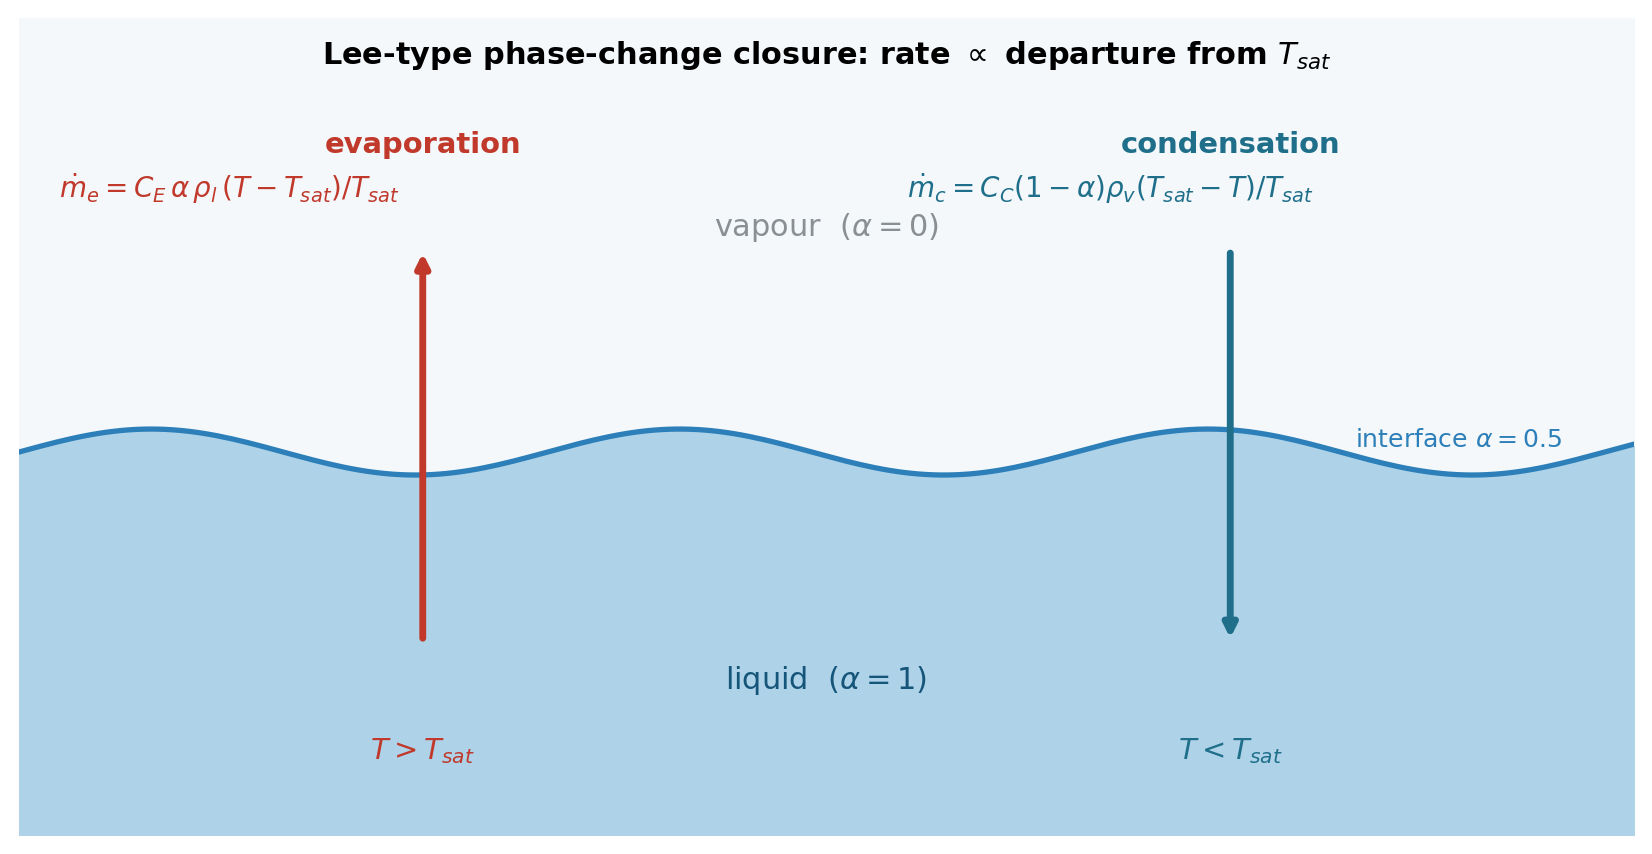
\includegraphics[width=0.84\textwidth]{fig_phasechange.png}
\caption{Phase-change closure: evaporation where the cell is superheated ($T>T_{sat}$) and
condensation where it is subcooled ($T<T_{sat}$), each at a rate proportional to the
departure from saturation. The interface is the $\alpha=0.5$ surface.}
\label{of-fig:pc}
\end{figure}

\subsection{Flow regime and dimensionless groups}
\label{of-sec:dimensionless}
Table~\ref{of-tab:dim} collects the governing dimensionless groups for water at the operating
point. Three features shape the modeling choices. First, the pool Rayleigh number
($\mathrm{Ra}\sim9\times10^6$, based on the liquid depth and the chip-to-pool difference)
sits well below the $\sim10^9$ transition for a heated horizontal layer, so the bulk
buoyant flow is laminar; the vigorous agitation in the chamber is driven by boiling and
bubble departure rather than by turbulent natural convection, which supports the laminar
mixture treatment with the interface resolved. Second, the Bond and confinement numbers
based on tube diameter ($\mathrm{Bo}=1.5$--$3.4$, $\mathrm{Co}=L_c/D=0.5$--$0.8$) show the
capillary length $L_c=\sqrt{\sigma/\rho_l g}\approx\SI{2.6}{mm}$ is comparable to the tube
spacing, so capillarity and confinement matter at the bundle, the smaller-bore confined
42-tube bundle is more strongly affected than the open 33-tube. Third, the liquid-to-vapor
density ratio is large ($\rho_l/\rho_v\approx3300$) and the superheat Jakob number is small
($\mathrm{Ja}=c_{p,l}\Delta T_{sup}/h_{fg}\approx0.04$); the large density ratio is the main
source of numerical stiffness (the volume source in Eq.~\eqref{of-eq:cont} and the property
jump), which is why the time step is interface-Courant limited. The chamber operates in
nucleate boiling up to CHF (Fig.~\ref{of-fig:regime}); the model is not intended for the
transition or film-boiling branches.

\begin{table}[H]
\centering\caption{Dimensionless groups (water, operating point: $\Delta T_{sup}\approx
\SI{20}{K}$, $\Delta T_{sub}\approx\SI{15}{K}$, liquid depth \SI{16.8}{mm}).}
\label{of-tab:dim}
\small
\begin{tabular}{llcl}
\toprule
Group & Definition & Value & Role\\
\midrule
Capillary length & $L_c=\sqrt{\sigma/\rho_l g}$ & \SI{2.6}{mm} & bubble / meniscus scale\\
Prandtl (liquid) & $\mu c_p/k$ & 2.7 & momentum vs thermal diffusion\\
Jakob (superheat) & $c_{p,l}\Delta T_{sup}/h_{fg}$ & 0.036 & sensible vs latent at the chip\\
Jakob (subcooling) & $c_{p,l}\Delta T_{sub}/h_{fg}$ & 0.027 & condensation driving\\
Density-ratio Jakob & $\rho_l c_{p,l}\Delta T_{sup}/(\rho_v h_{fg})$ & 117 & vapour generation intensity\\
Bond (42 / 33-tube) & $\rho_l g\,D^2/\sigma$ & 1.5 / 3.4 & gravity vs capillarity at a tube\\
Confinement (42 / 33) & $L_c/D$ & 0.82 / 0.55 & bundle confinement\\
Rayleigh (pool) & $g\beta\Delta T H^3/\nu\alpha_{th}$ & $9\times10^6$ & laminar bulk convection\\
Density ratio & $\rho_l/\rho_v$ & 3300 & numerical stiffness\\
\bottomrule
\end{tabular}
\end{table}

\begin{figure}[H]
\centering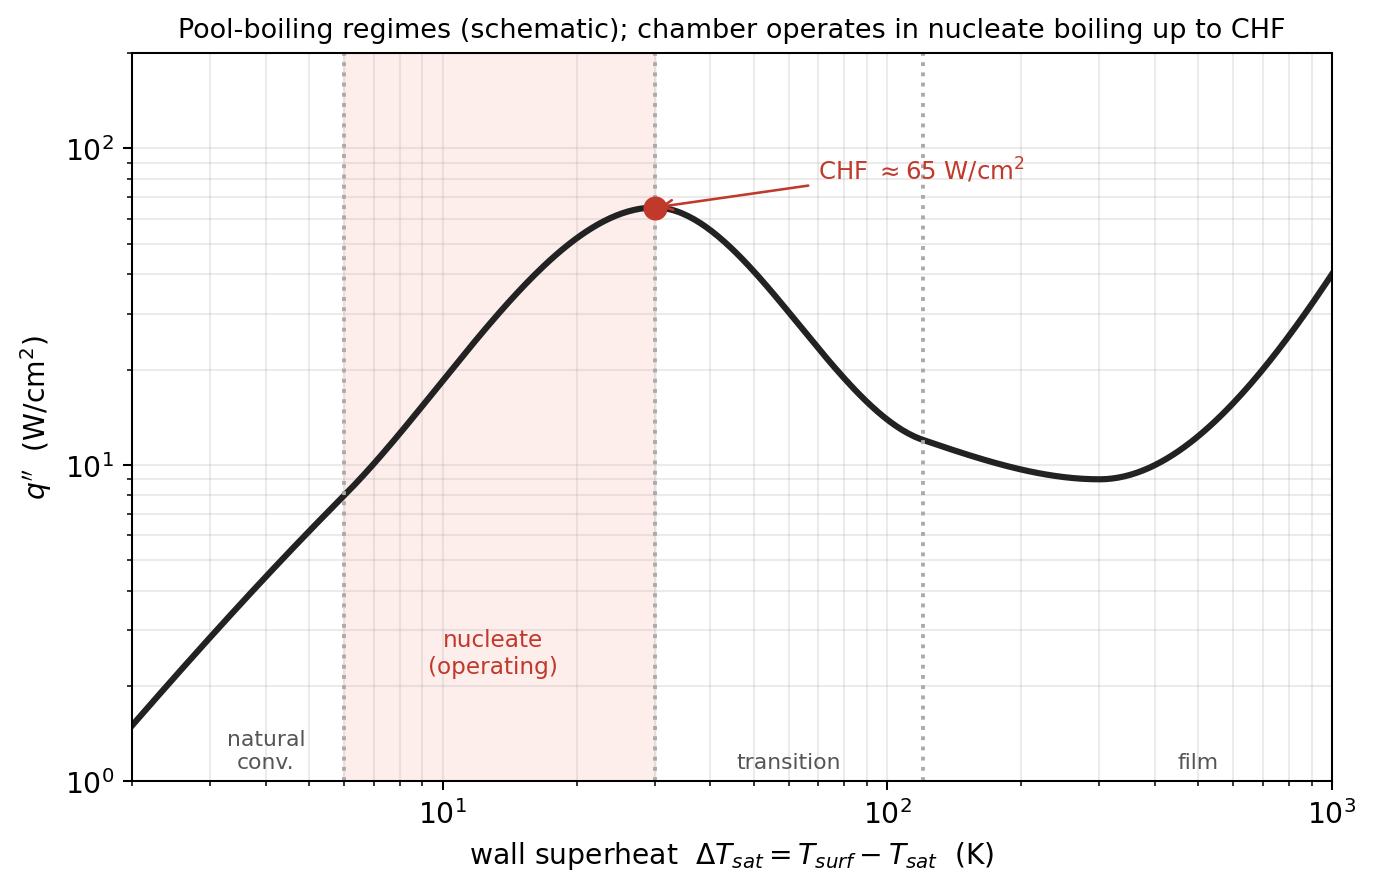
\includegraphics[width=0.72\textwidth]{fig_regime.png}
\caption{Pool-boiling regime map (schematic). The chamber operates on the nucleate-boiling
branch up to the measured CHF; the constant-coefficient closure is calibrated for this
branch, not for transition or film boiling.}
\label{of-fig:regime}
\end{figure}

\section{Mesh generation}
\label{of-sec:mesh}
A structured background grid (\texttt{blockMesh}, $40\times40\times21$, \num{33600}
cells) is refined with \texttt{snappyHexMesh}: surface refinement and feature snapping on
the tubes, refinement boxes over the chip and bundle, and prism layers. The chip patch is
cut from the floor. Body-fitted meshing of all 42 tubes is verified
(Fig.~\ref{of-fig:meshref}): snapping yields a complete grid of \num{299656} cells passing
\texttt{checkMesh} (max skewness \num{1.57}, 100\% layer addition), confirming the
limitation to a fully refined grid is cost, not mesh validity (Table~\ref{of-tab:mesh}).

\begin{figure}[H]
\centering
\begin{subfigure}{0.99\textwidth}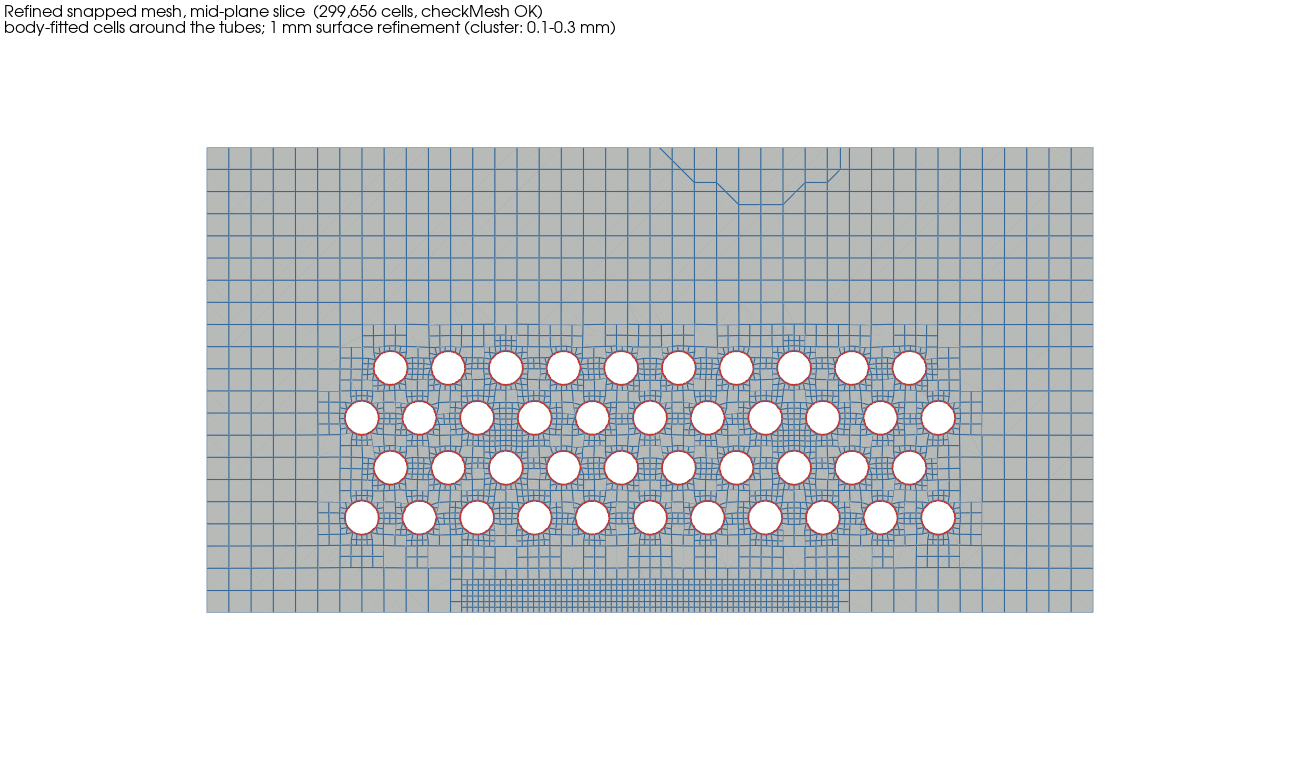
\includegraphics[width=\textwidth]{refined_mesh_slice.png}
\caption{Mid-plane slice: body-fitted cells with graded refinement and the chip box.}
\end{subfigure}\\[4pt]
\begin{subfigure}{0.78\textwidth}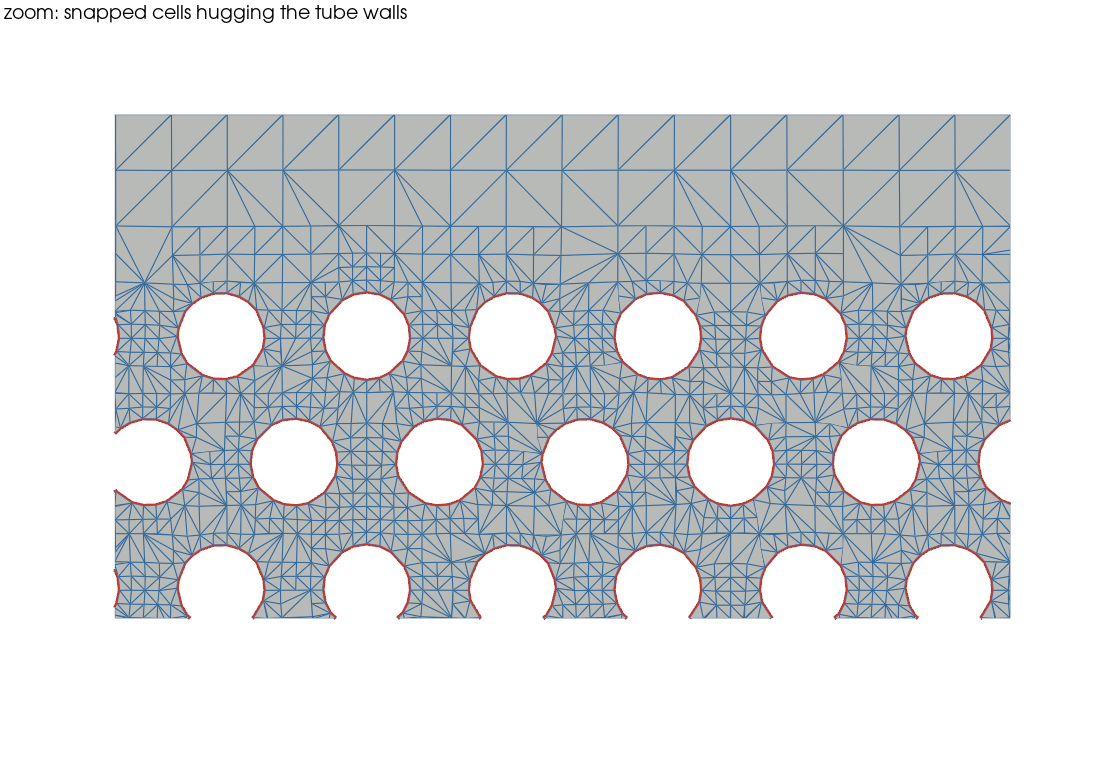
\includegraphics[width=\textwidth]{refined_mesh_zoom.png}
\caption{Detail at the tube walls.}\end{subfigure}
\caption{Verified body-fitted snapped mesh (\num{299656} cells, \texttt{checkMesh} OK).}
\label{of-fig:meshref}
\end{figure}

\begin{table}[H]
\centering\caption{Mesh states.}\label{of-tab:mesh}
\begin{tabular}{lccl}
\toprule
Mesh & Construction & Cells & Notes\\
\midrule
Background & \texttt{blockMesh} & \num{33600} & $\sim$\SI{2}{mm}\\
Demonstration & castellation-only & \num{74044} & staircased, robust\\
Verified snapped & snap, level $(1\,2)$ & \num{299656} & \texttt{checkMesh} OK, skew \num{1.57}\\
Production target & shipped dict & $\sim$few$\times10^6$ & \SIrange{0.1}{0.3}{mm}, snap + layers\\
\bottomrule
\end{tabular}
\end{table}

\section{Boundary, initial, and coolant operating conditions}
\label{of-sec:bc}
The chip is a fixed-temperature wall and the condenser tubes a colder fixed-temperature
wall; remaining walls are adiabatic no-slip, $T_{sat}=\SI{338}{K}$, and the pool is
initialized below \SI{16.8}{mm} (Fig.~\ref{of-fig:bc}, Table~\ref{of-tab:bc}). These wall
temperatures are representative; the calibration matches the simulated boiling curve to
the measured one (Section~\ref{of-sec:reference}).

\begin{figure}[H]
\centering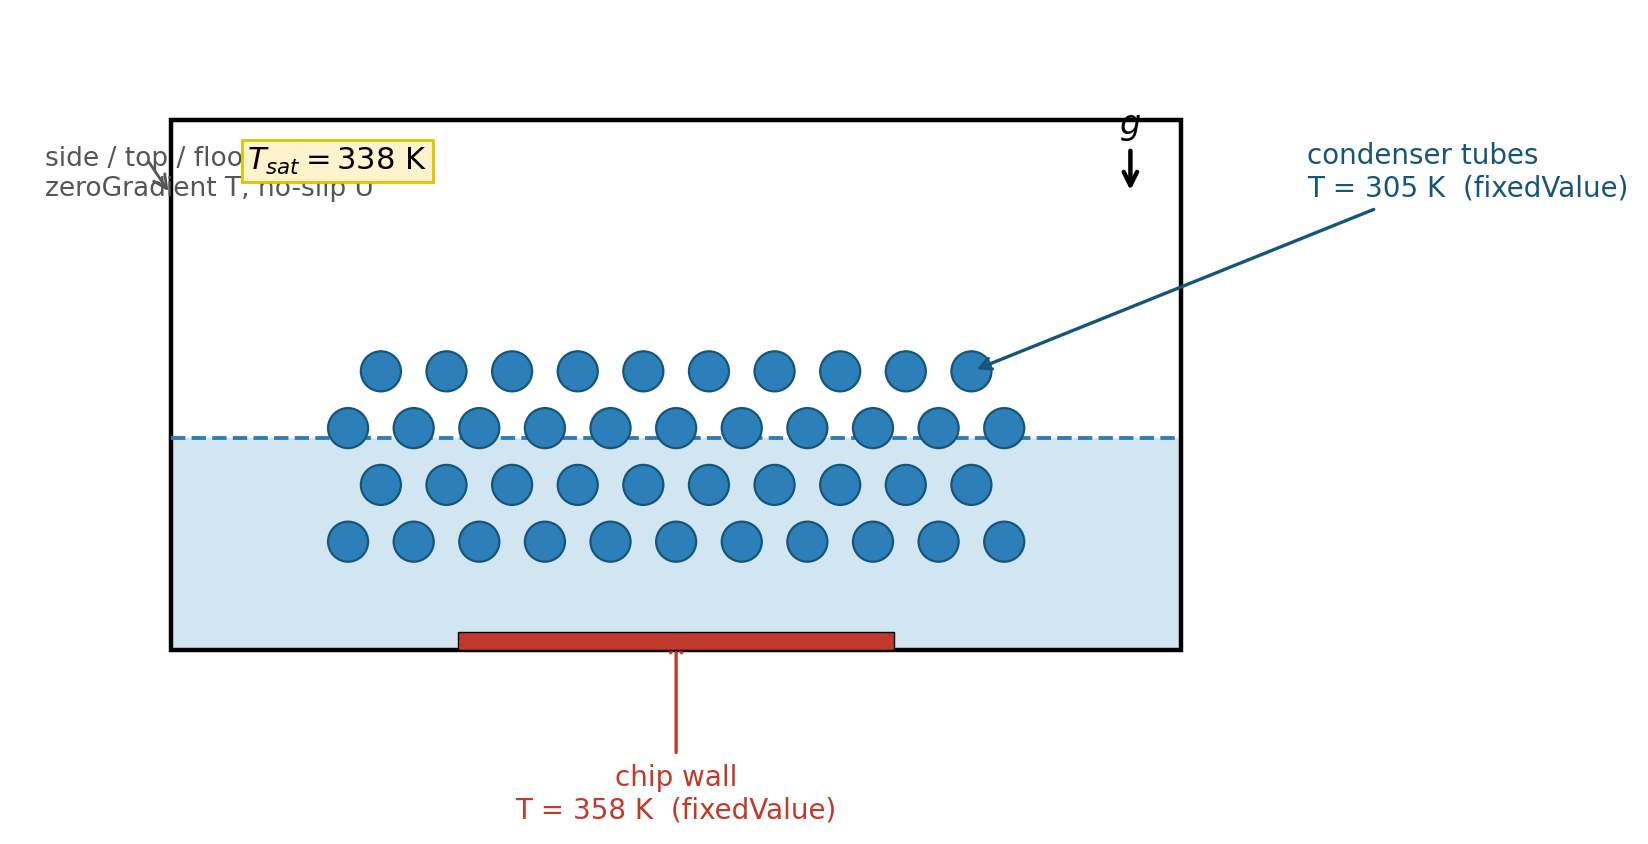
\includegraphics[width=0.72\textwidth]{fig_bc.png}
\caption{Boundary and initial conditions on the $x$--$z$ cross-section.}
\label{of-fig:bc}
\end{figure}

\begin{table}[H]
\centering\caption{Field boundary conditions.}\label{of-tab:bc}
\begin{tabular}{llll}
\toprule
Patch & $T$ & $\mathbf U$ & $p_{rgh}$\\
\midrule
chip & fixedValue \SI{358}{K} & noSlip & fixedFluxPressure\\
condenser & fixedValue \SI{305}{K} & noSlip & fixedFluxPressure\\
floor / walls / top & zeroGradient & noSlip & fixedFluxPressure\\
\midrule
\multicolumn{4}{l}{Internal $T=\SI{325}{K}$, $\mathbf U=0$, $\alpha$ from
\texttt{setFields}; $T_{sat}=\SI{338}{K}$.}\\
\bottomrule
\end{tabular}
\end{table}

\noindent\textbf{Condenser coolant operating point (measured).} The condenser tubes
carry single-phase water coolant; its measured operating conditions set the cold-side
boundary that the fixed-temperature wall idealizes. Table~\ref{of-tab:coolant} reports the
inlet and outlet temperatures, mass flow, the resulting per-tube velocity and Reynolds
number, and the chamber pressure for both condensers across the four coolant set points.
The flow is laminar and developing in both bundles ($\mathrm{Re}\sim700$--$1600$); the
42-tube bundle runs at higher velocity (smaller bore) and lower chamber pressure at the
warm set points. The coolant temperature rise $T_{out}-T_{in}$ is the calorimetric basis
for the condenser duty $Q=\dot m c_p (T_{out}-T_{in})$.

\begin{table}[H]
\centering\caption{Measured condenser coolant conditions (per coolant set point; values
are run-averaged). $V$ and $\mathrm{Re}$ are per-tube, evaluated at $T_{in}$.}
\label{of-tab:coolant}
\footnotesize
\begin{tabular}{llcccccc}
\toprule
Bundle, chip & Set & $T_{in}$ (\si{\celsius}) & $T_{out}$ (\si{\celsius}) &
$\Delta T$ (K) & $\dot m$ (g/s) & $V$ (m/s) & $\mathrm{Re}$\\
\midrule
33, plain & 20 & 20.0 & 21.7 & 1.7 & 60.0 & 0.235 & 735\\
          & 30 & 29.2 & 31.0 & 1.8 & 60.0 & 0.236 & 910\\
          & 40 & 39.4 & 41.0 & 1.6 & 60.0 & 0.237 & 1116\\
          & 50 & 48.3 & 49.9 & 1.6 & 60.0 & 0.237 & 1310\\
33, micro & 20 & 20.2 & 23.3 & 3.1 & 62.5 & 0.245 & 771\\
          & 40 & 40.9 & 44.4 & 3.4 & 62.5 & 0.247 & 1197\\
42, plain & 20 & 20.0 & 22.1 & 2.1 & 38.8 & 0.610 & 845\\
          & 30 & 30.0 & 32.5 & 2.5 & 38.8 & 0.611 & 1061\\
          & 40 & 40.1 & 42.2 & 2.2 & 38.8 & 0.614 & 1298\\
          & 50 & 50.0 & 52.0 & 2.0 & 38.8 & 0.616 & 1549\\
42, micro & 20 & 20.0 & 23.5 & 3.5 & 41.0 & 0.644 & 893\\
          & 30 & 29.9 & 34.5 & 4.5 & 38.8 & 0.611 & 1060\\
          & 40 & 40.0 & 44.3 & 4.3 & 38.8 & 0.614 & 1296\\
          & 50 & 49.9 & 54.9 & 5.0 & 38.8 & 0.616 & 1547\\
\bottomrule
\end{tabular}\\[2pt]
\footnotesize Chamber pressure ranges \SIrange{72}{85}{kPa} (33-tube) and
\SIrange{37}{85}{kPa} (42-tube), falling at the warm set points as $T_{sat}$ drops.
\end{table}

\section{Material properties and numerics}
\label{of-sec:numerics}
Properties are in Table~\ref{of-tab:props}; the phase-change coefficients are the
uncalibrated placeholders $C_C=1.0$, $C_E=0.1$. Time integration is Euler with an
adjustable step ($\mathrm{Co}\le0.4$); convection uses \texttt{linearUpwind} (momentum,
energy) and \texttt{vanLeer} with interface compression for $\alpha$; pressure uses
PCG/DIC, $\alpha$ uses MULES, within a PISO loop (Table~\ref{of-tab:run}).

\begin{table}[H]
\centering
\begin{minipage}[t]{0.54\textwidth}\centering\caption{Material properties.}\label{of-tab:props}\small
\begin{tabular}{lccc}
\toprule
Property & Water & Vapor & Unit\\\midrule
$\rho$ & 980 & 0.30 & \si{kg/m^3}\\
$\nu$ & \num{4.4e-7} & \num{4.0e-4} & \si{m^2/s}\\
$c_p$ & 4190 & 2030 & \si{J/kg/K}\\
$\kappa$ & 0.66 & 0.025 & \si{W/m/K}\\
$h_{fg}$ & & \num{2.35e6} & \si{J/kg}\\\midrule
\multicolumn{4}{l}{$\sigma=\SI{0.065}{N/m}$, $Pr_t=1.0$, laminar}\\
\bottomrule
\end{tabular}\end{minipage}\hfill
\begin{minipage}[t]{0.42\textwidth}\centering\caption{Run control.}\label{of-tab:run}\small
\begin{tabular}{ll}
\toprule
Setting & Value\\\midrule
$\Delta t$ & \SI{1e-6}{s}\\
$\mathrm{Co},\mathrm{Co}_\alpha$ & $\le0.4$\\
end (demo) & \SI{8e-4}{s}\\
$\alpha$ & MULES, $c_\alpha=1$\\
$p_{rgh}$ & PCG/DIC\\
PISO & 2 correctors\\
$C_C,C_E$ & 1.0,\,0.1 (uncal.)\\
\bottomrule
\end{tabular}\end{minipage}
\end{table}

\section{Reference data and the validation target}
\label{of-sec:reference}
This section assembles what the CFD must reproduce. \textbf{The curves and resistances
here are measured data and the validated reduced-order model of the same apparatus, not
CFD output.} They define the envelope against which the converged CFD
(Section~\ref{of-sec:post}) will be judged.

\subsection{Measured boiling curves and the reduced-order model}
Figure~\ref{of-fig:boil} overlays the measured boiling curves (points) with the reduced-order
model (lines) for both condensers and both chips across coolant set points. The model
tracks the data with a per-configuration RMS error of \SIrange{3.1}{5.2}{K} in surface
temperature. The microchannel surface boils at markedly lower superheat than the plain
surface at the same flux, and the 33-tube condenser reaches higher flux at a given surface
temperature than the confined 42-tube. These are the trends, and the absolute curves,
the 3D simulation is required to recover.

\begin{figure}[H]
\centering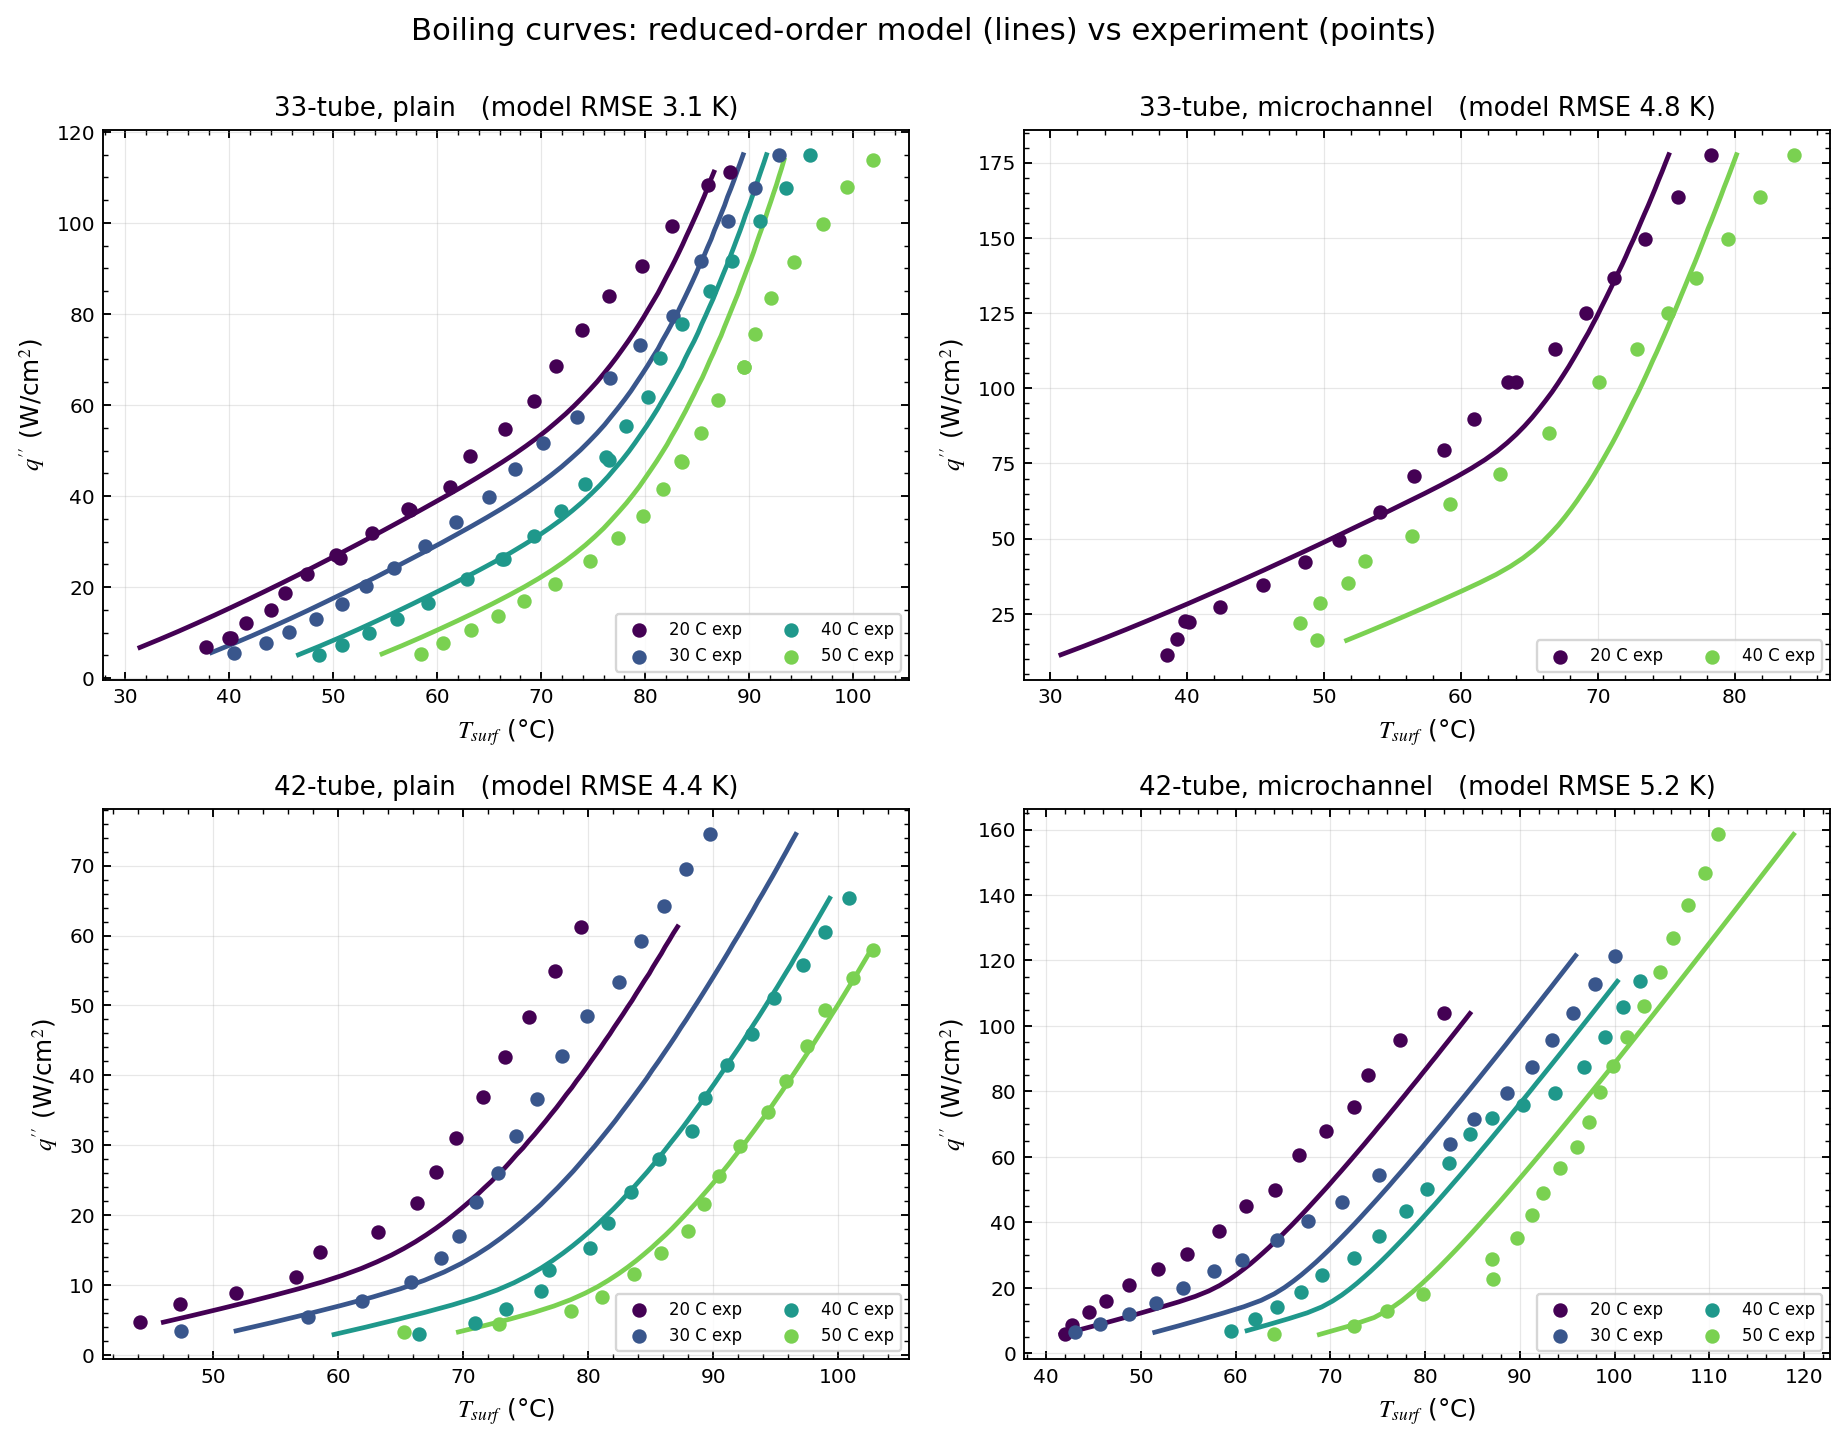
\includegraphics[width=0.95\textwidth]{fig_boiling_overlay.png}
\caption{Boiling curves: reduced-order model (lines) vs experiment (points) for both
condensers and both chips, colored by coolant inlet temperature. \emph{Reference data and
validated reduced-order model; not CFD output.}}
\label{of-fig:boil}
\end{figure}

\subsection{Thermal resistance}
The chip-to-coolant path is summarized by the total resistance
$R_{tot}=(T_{surf}-T_{in})/Q$, split into a boiling (chip-side) resistance
$R_{chip}=(T_{surf}-T_{liq})/Q$ and a pool-to-coolant (condenser-side) resistance
$R_{cond}=(T_{liq}-T_{in})/Q$. Figure~\ref{of-fig:res} shows $R_{tot}$ versus heat flux from
experiment and from the reduced-order model; Table~\ref{of-tab:res} lists the median
breakdown. Two results stand out. First, the condenser-side resistance is far smaller for
the open 33-tube bundle (\SIrange{14}{15}{mK/W}) than for the confined 42-tube bundle
(\SIrange{41}{74}{mK/W}), consistent with the open bundle being coolant-side limited and
the confined bundle carrying a layout penalty. Second, the microchannel surface roughly
halves the chip-side resistance relative to plain (e.g. 17 vs \SI{64}{mK/W} on the
33-tube), which is the resistance signature of its lower boiling superheat. The
reduced-order model reproduces $R_{tot}$ to within a few \si{mK/W} except for the 33-tube
microchannel, where it over-predicts (44 vs \SI{33}{mK/W}), the same configuration that
carries the largest boiling-curve error.

\begin{figure}[H]
\centering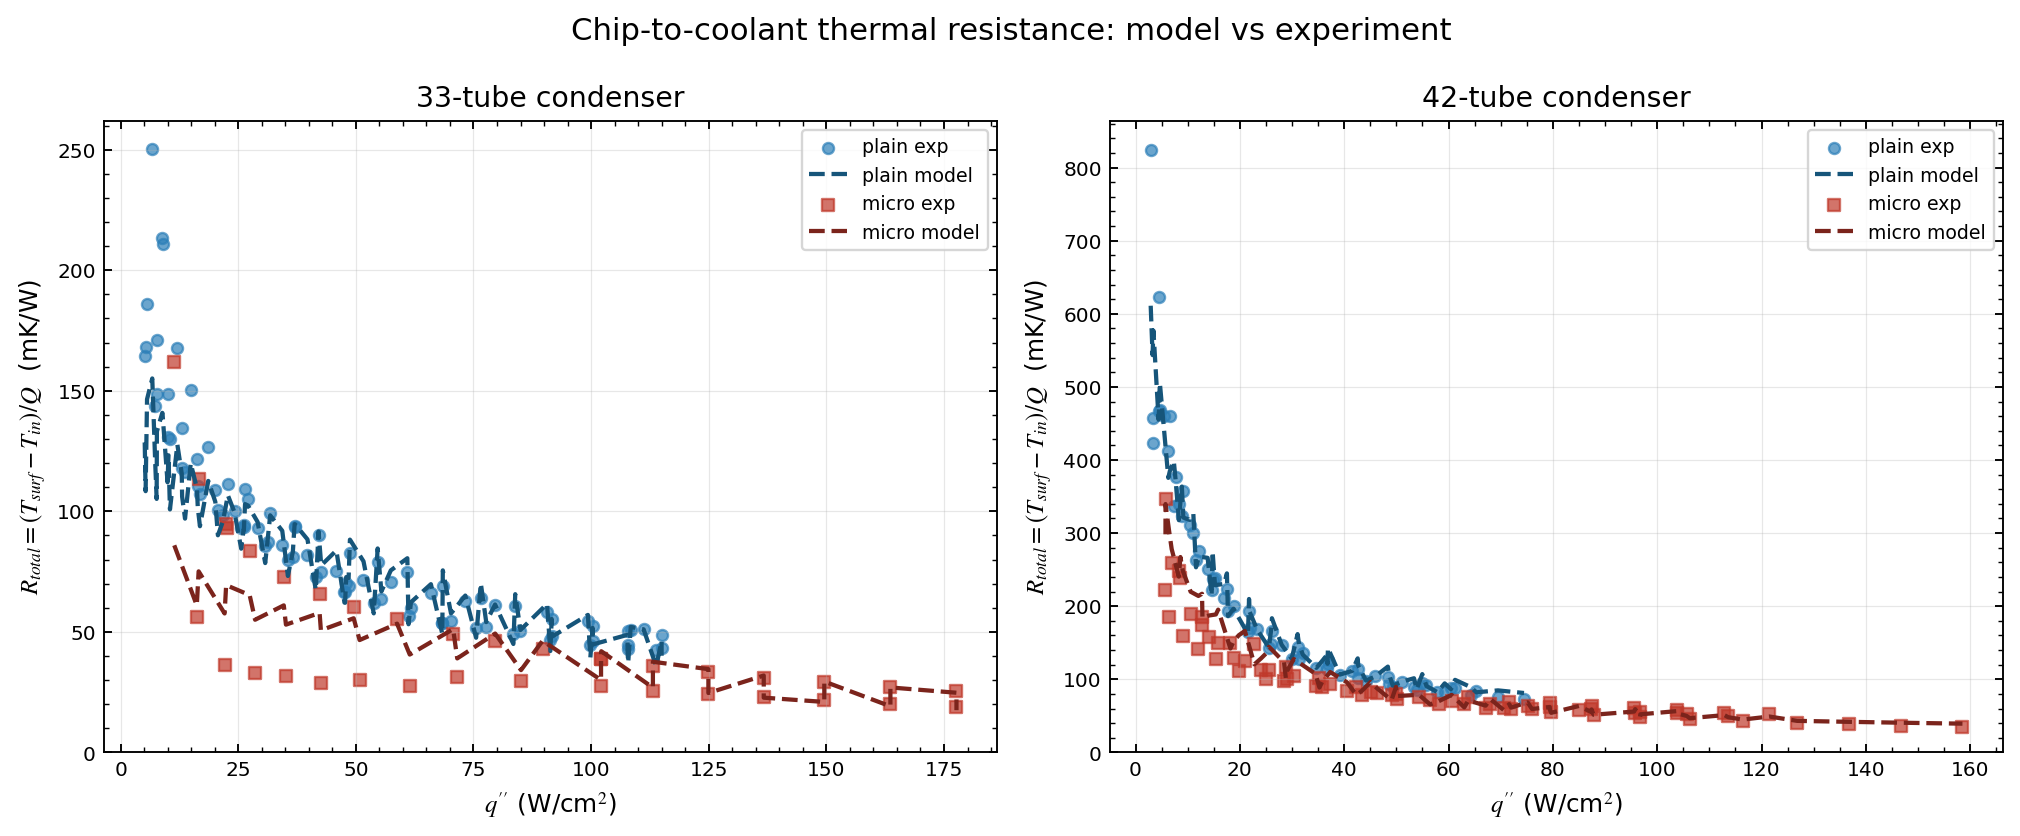
\includegraphics[width=0.92\textwidth]{fig_resistance.png}
\caption{Total chip-to-coolant resistance $R_{tot}=(T_{surf}-T_{in})/Q$ vs heat flux:
experiment (markers) and reduced-order model (dashed), per condenser.
\emph{Not CFD output.}}
\label{of-fig:res}
\end{figure}

\begin{table}[H]
\centering\caption{Median thermal resistance breakdown (\si{mK/W}). $R_{tot}$ is shown for
experiment and the reduced-order model; the experimental split into $R_{chip}$ and
$R_{cond}$ is from $(T_{surf}-T_{liq})$ and $(T_{liq}-T_{in})$.}
\label{of-tab:res}
\begin{tabular}{lcccc}
\toprule
Configuration & $R_{tot}$ exp & $R_{tot}$ model & $R_{chip}$ exp & $R_{cond}$ exp\\
\midrule
33-tube, plain        & 78.9  & 80.5  & 64.4 & 13.7\\
33-tube, microchannel & 33.1  & 44.1  & 17.3 & 15.1\\
42-tube, plain        & 148.2 & 161.9 & 75.1 & 74.0\\
42-tube, microchannel & 77.1  & 78.7  & 31.9 & 41.1\\
\bottomrule
\end{tabular}
\end{table}

\subsection{Calibration workflow and CHF}
The constant-coefficient closure carries two coefficients that must be calibrated against
data (Fig.~\ref{of-fig:workflow}). Calibration sweeps the chip wall temperature for each
candidate $(C_E,C_C)$, builds the simulated boiling curve from a chip-patch heat-flux
probe ($k_{\mathrm{eff}}=\alpha k_w+(1-\alpha)k_v$), and minimizes the RMS misfit to the
measured curve plus a CHF turn-over penalty. The 42-tube/plain target is 64 measured
points across four coolant temperatures with a measured CHF of \SI{65}{W/cm^2}
(Fig.~\ref{of-fig:val}).

\begin{figure}[H]
\centering
\begin{subfigure}{0.62\textwidth}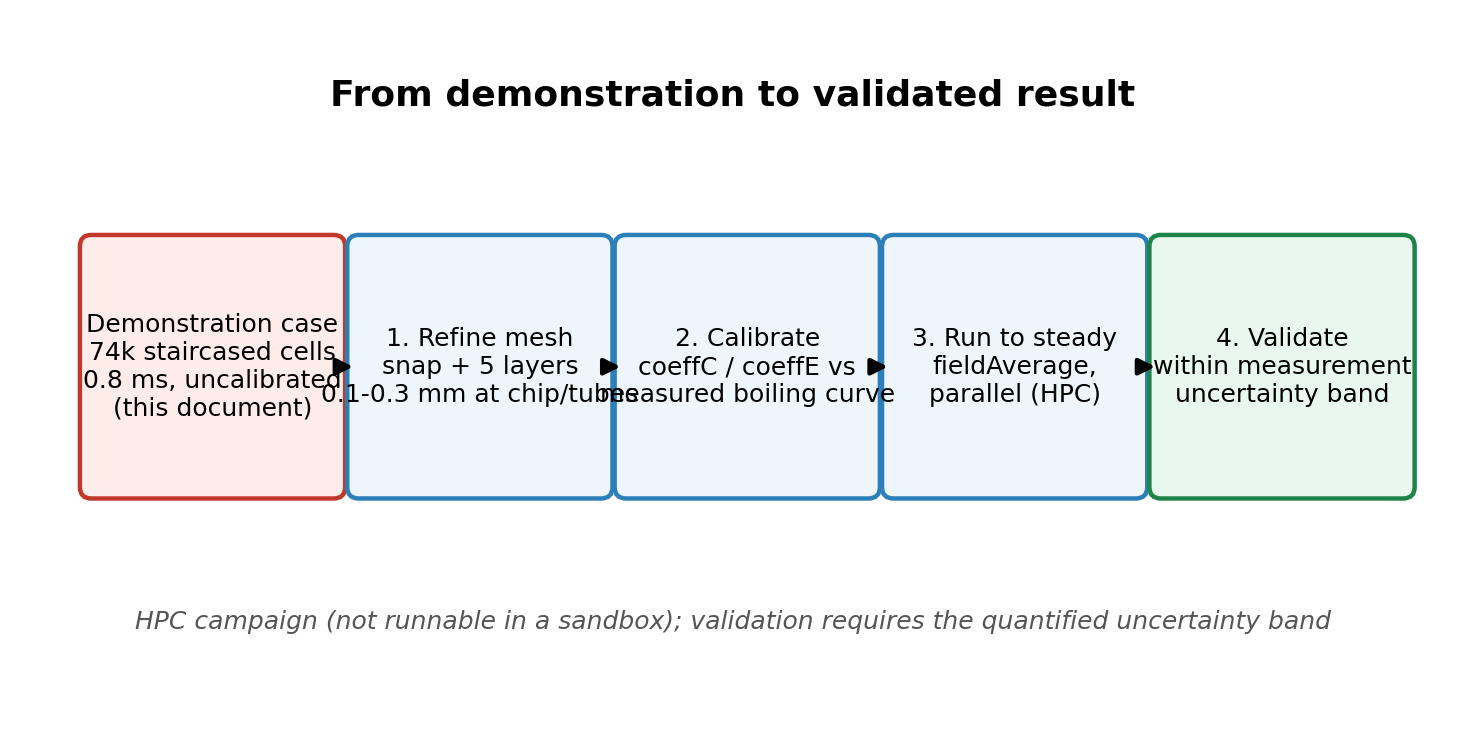
\includegraphics[width=\textwidth]{fig_workflow.png}
\caption{Refine $\rightarrow$ calibrate $\rightarrow$ run $\rightarrow$ validate.}
\end{subfigure}\hfill
\begin{subfigure}{0.36\textwidth}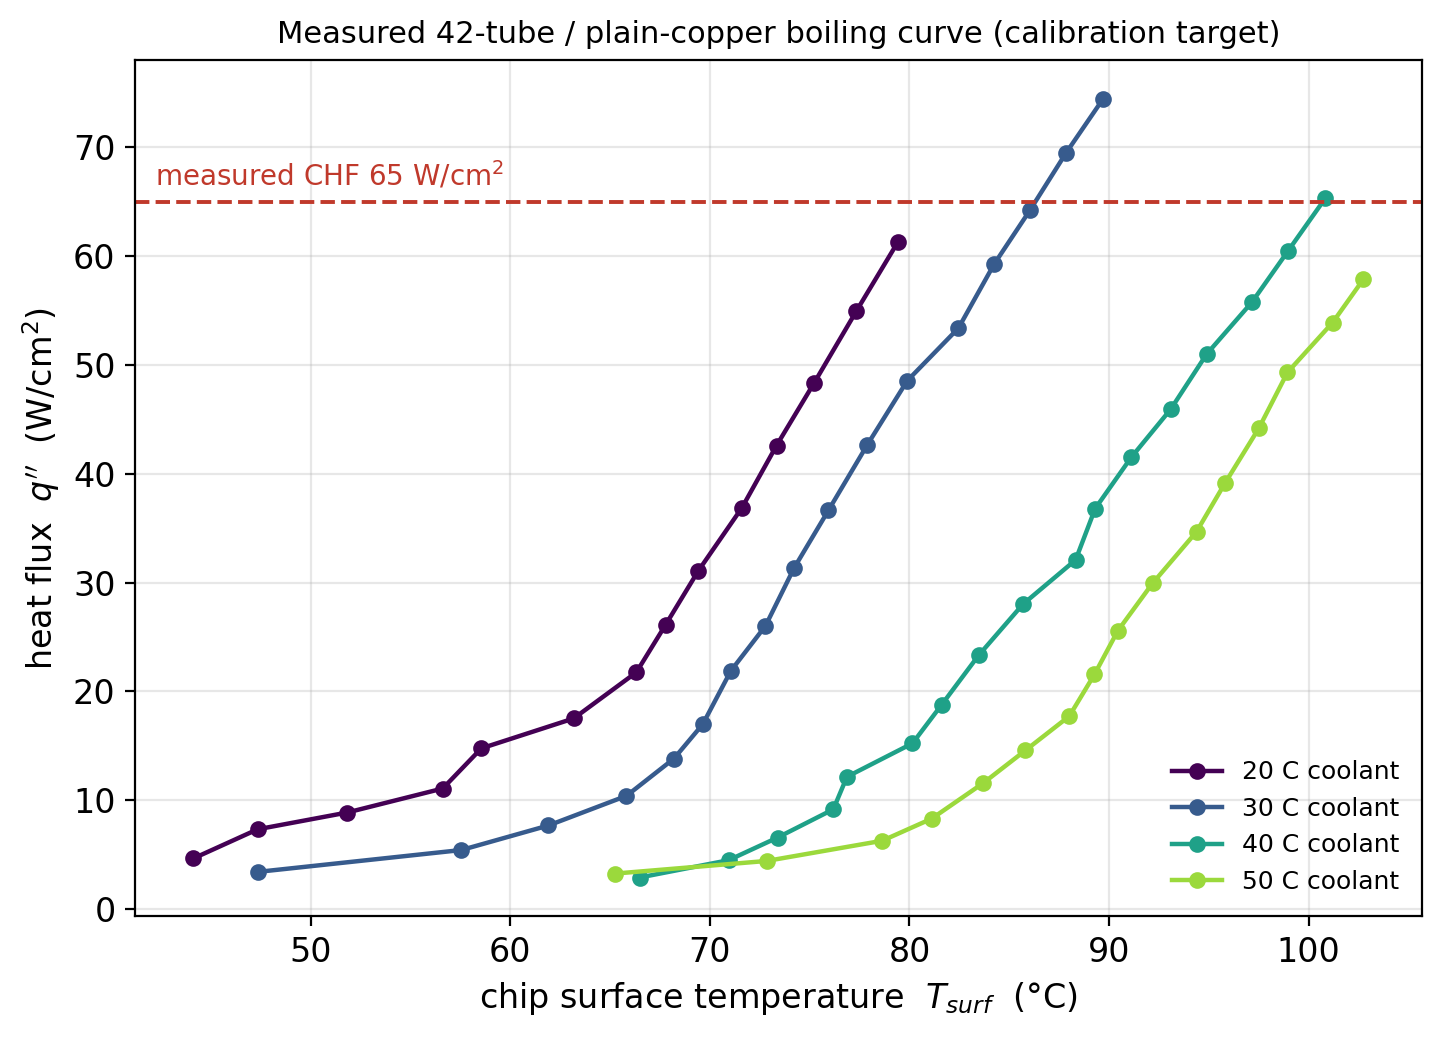
\includegraphics[width=\textwidth]{fig_validation.png}
\caption{42-tube/plain target.}\end{subfigure}
\caption{Calibration-to-validation workflow and the measured 42-tube/plain calibration
target (CHF \SI{65}{W/cm^2}).}
\label{of-fig:workflow}\label{of-fig:val}
\end{figure}

\section{Condenser coolant-side flow routing and thermal-hydraulics}
\label{of-sec:coolant}
The two condensers route the single-phase coolant differently, which shapes the cold-side
boundary that the fixed-temperature tube walls idealize. The 33-tube bundle uses an open
manifold with a single parallel pass: coolant enters a header spanning the bundle,
distributes across all tubes, flows along the tube axis, and collects at the outlet header.
The 42-tube bundle uses a confined manifold: coolant enters from the top, descends into the
inlet manifold, passes through the tubes along their length, and returns up to the top
through the outlet manifold (Figs.~\ref{of-fig:cooltop} and~\ref{of-fig:coolside}).

The figures show the coolant temperature along the flow path, computed from a
one-dimensional energy balance on the measured condenser duty (Table~\ref{of-tab:coolant}):
the coolant warms from the measured inlet to outlet temperature as it absorbs the condenser
heat load, shown here at the \SI{20}{\celsius}, plain-chip operating point so the two
bundles share an inlet. \textbf{These are coolant-side thermal-hydraulic estimates on the
real geometry, not resolved CFD fields}; in the VOF case the tubes are fixed-temperature
walls and the coolant interior is not simulated. The temperature rise is modest in a single
pass (\SI{1.7}{K} for the 33-tube, \SI{2.1}{K} for the 42-tube at this point, the latter
warmer at outlet because its flow is lower, Table~\ref{of-tab:coolant}) and scales with heat
load, reaching about \SI{5}{K} for the 42-tube microchannel near CHF.

\begin{figure}[H]
\centering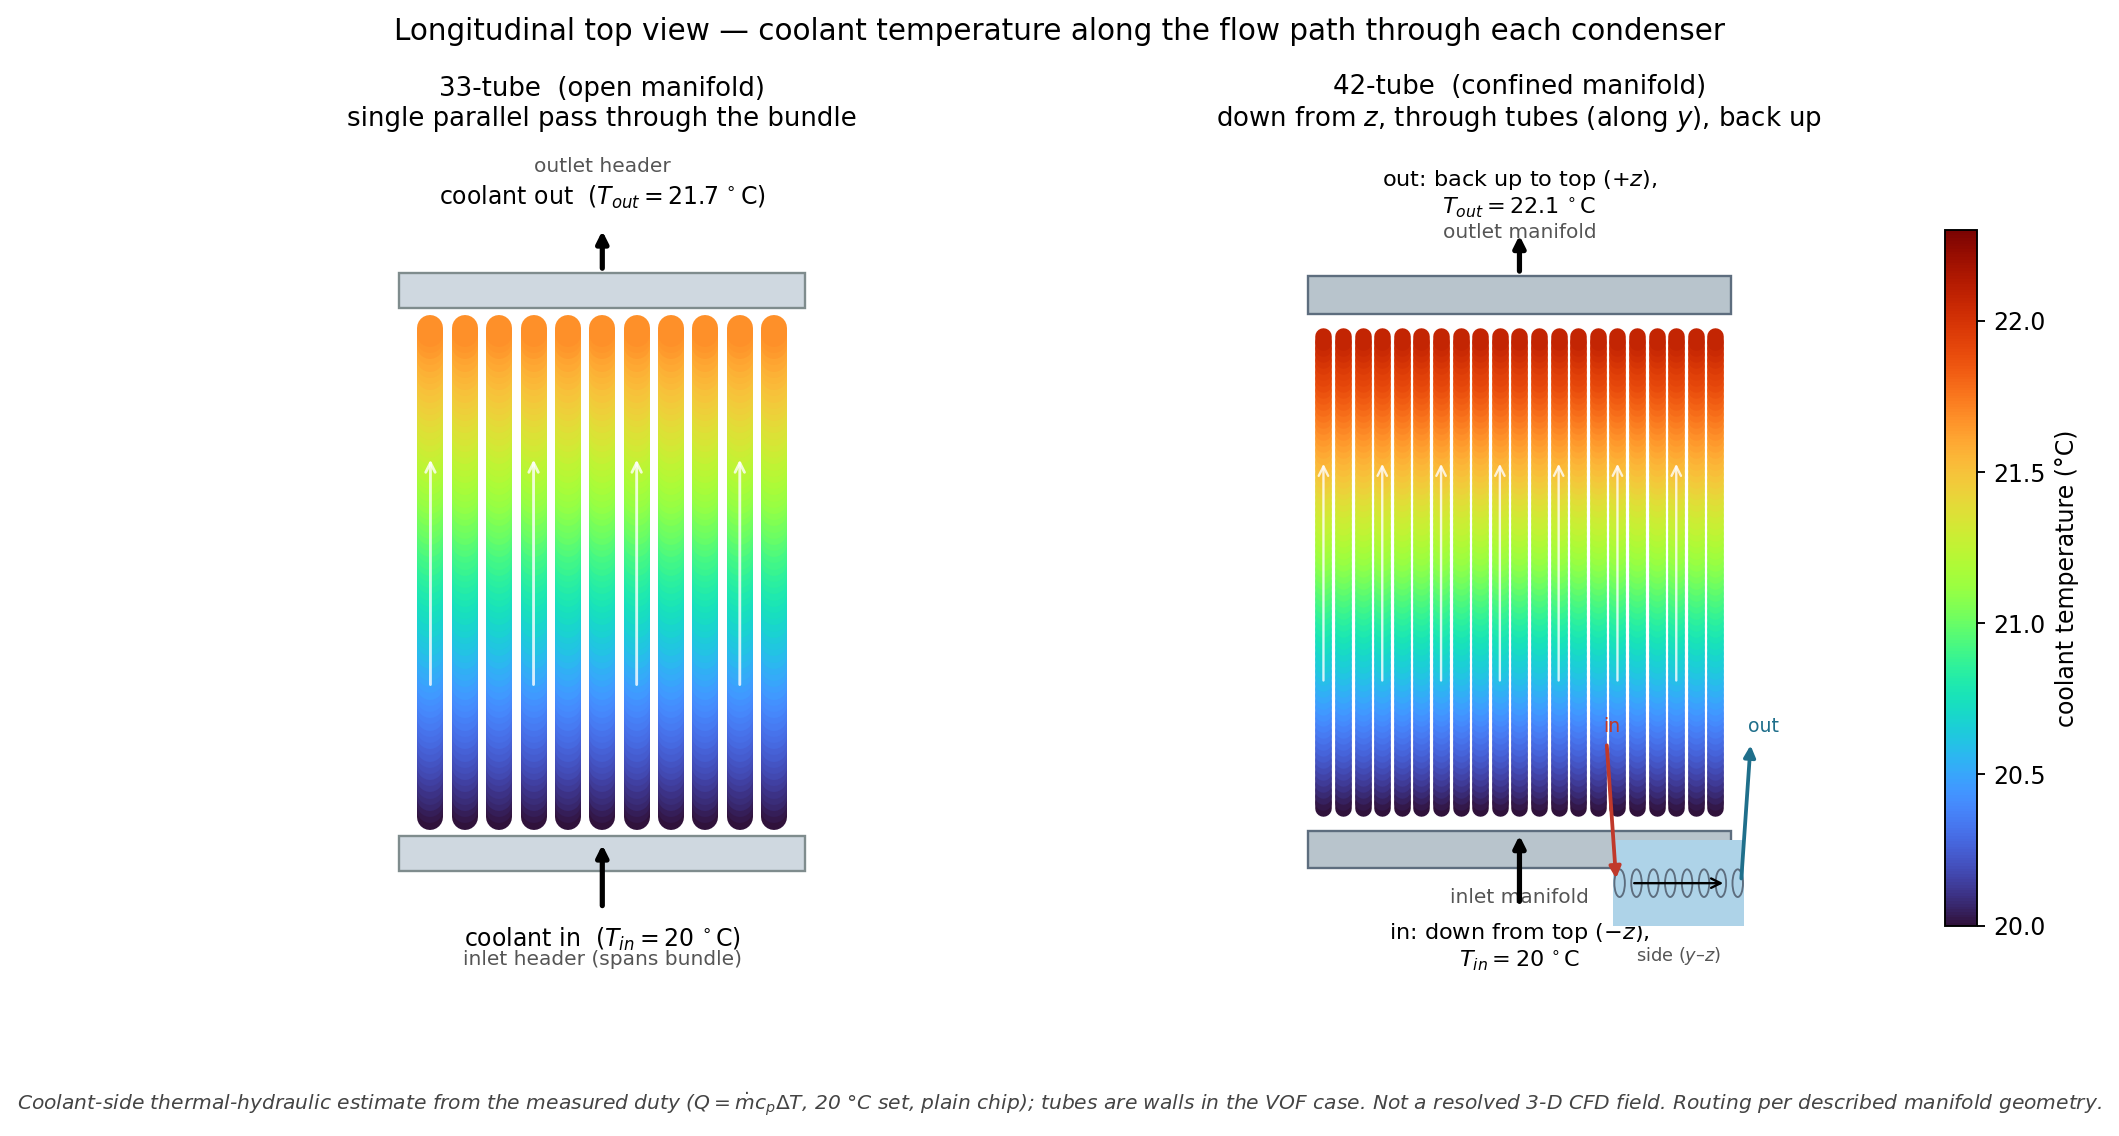
\includegraphics[width=0.96\textwidth]{fig_coolant_topview.png}
\caption{Longitudinal top view: coolant temperature along the flow path. The 33-tube (open
manifold) makes a single parallel pass; the 42-tube (confined manifold) enters from the top,
runs through the tubes, and returns up (side $y$--$z$ inset). \emph{Coolant-side
thermal-hydraulic estimate from the measured duty; not a resolved CFD field.}}
\label{of-fig:cooltop}
\end{figure}

The top view (Fig.~\ref{of-fig:cooltop}) shows the longitudinal warming along the tube axis. The
side view (Fig.~\ref{of-fig:coolside}, left column) contrasts the in-plane single pass of the
open 33-tube bundle with the down-through-up routing of the confined 42-tube. The end
cross-sections (Fig.~\ref{of-fig:coolside}, right column) show the bundle packing, the real
four-row, 21-column staggered 42-tube layout and the schematic three-row 33-tube, with the
inlet-to-outlet temperature difference. Resolving the coolant-side velocity, pressure drop,
and header maldistribution would require a separate internal-flow or conjugate simulation
(Section~\ref{of-sec:next}).

\begin{figure}[H]
\centering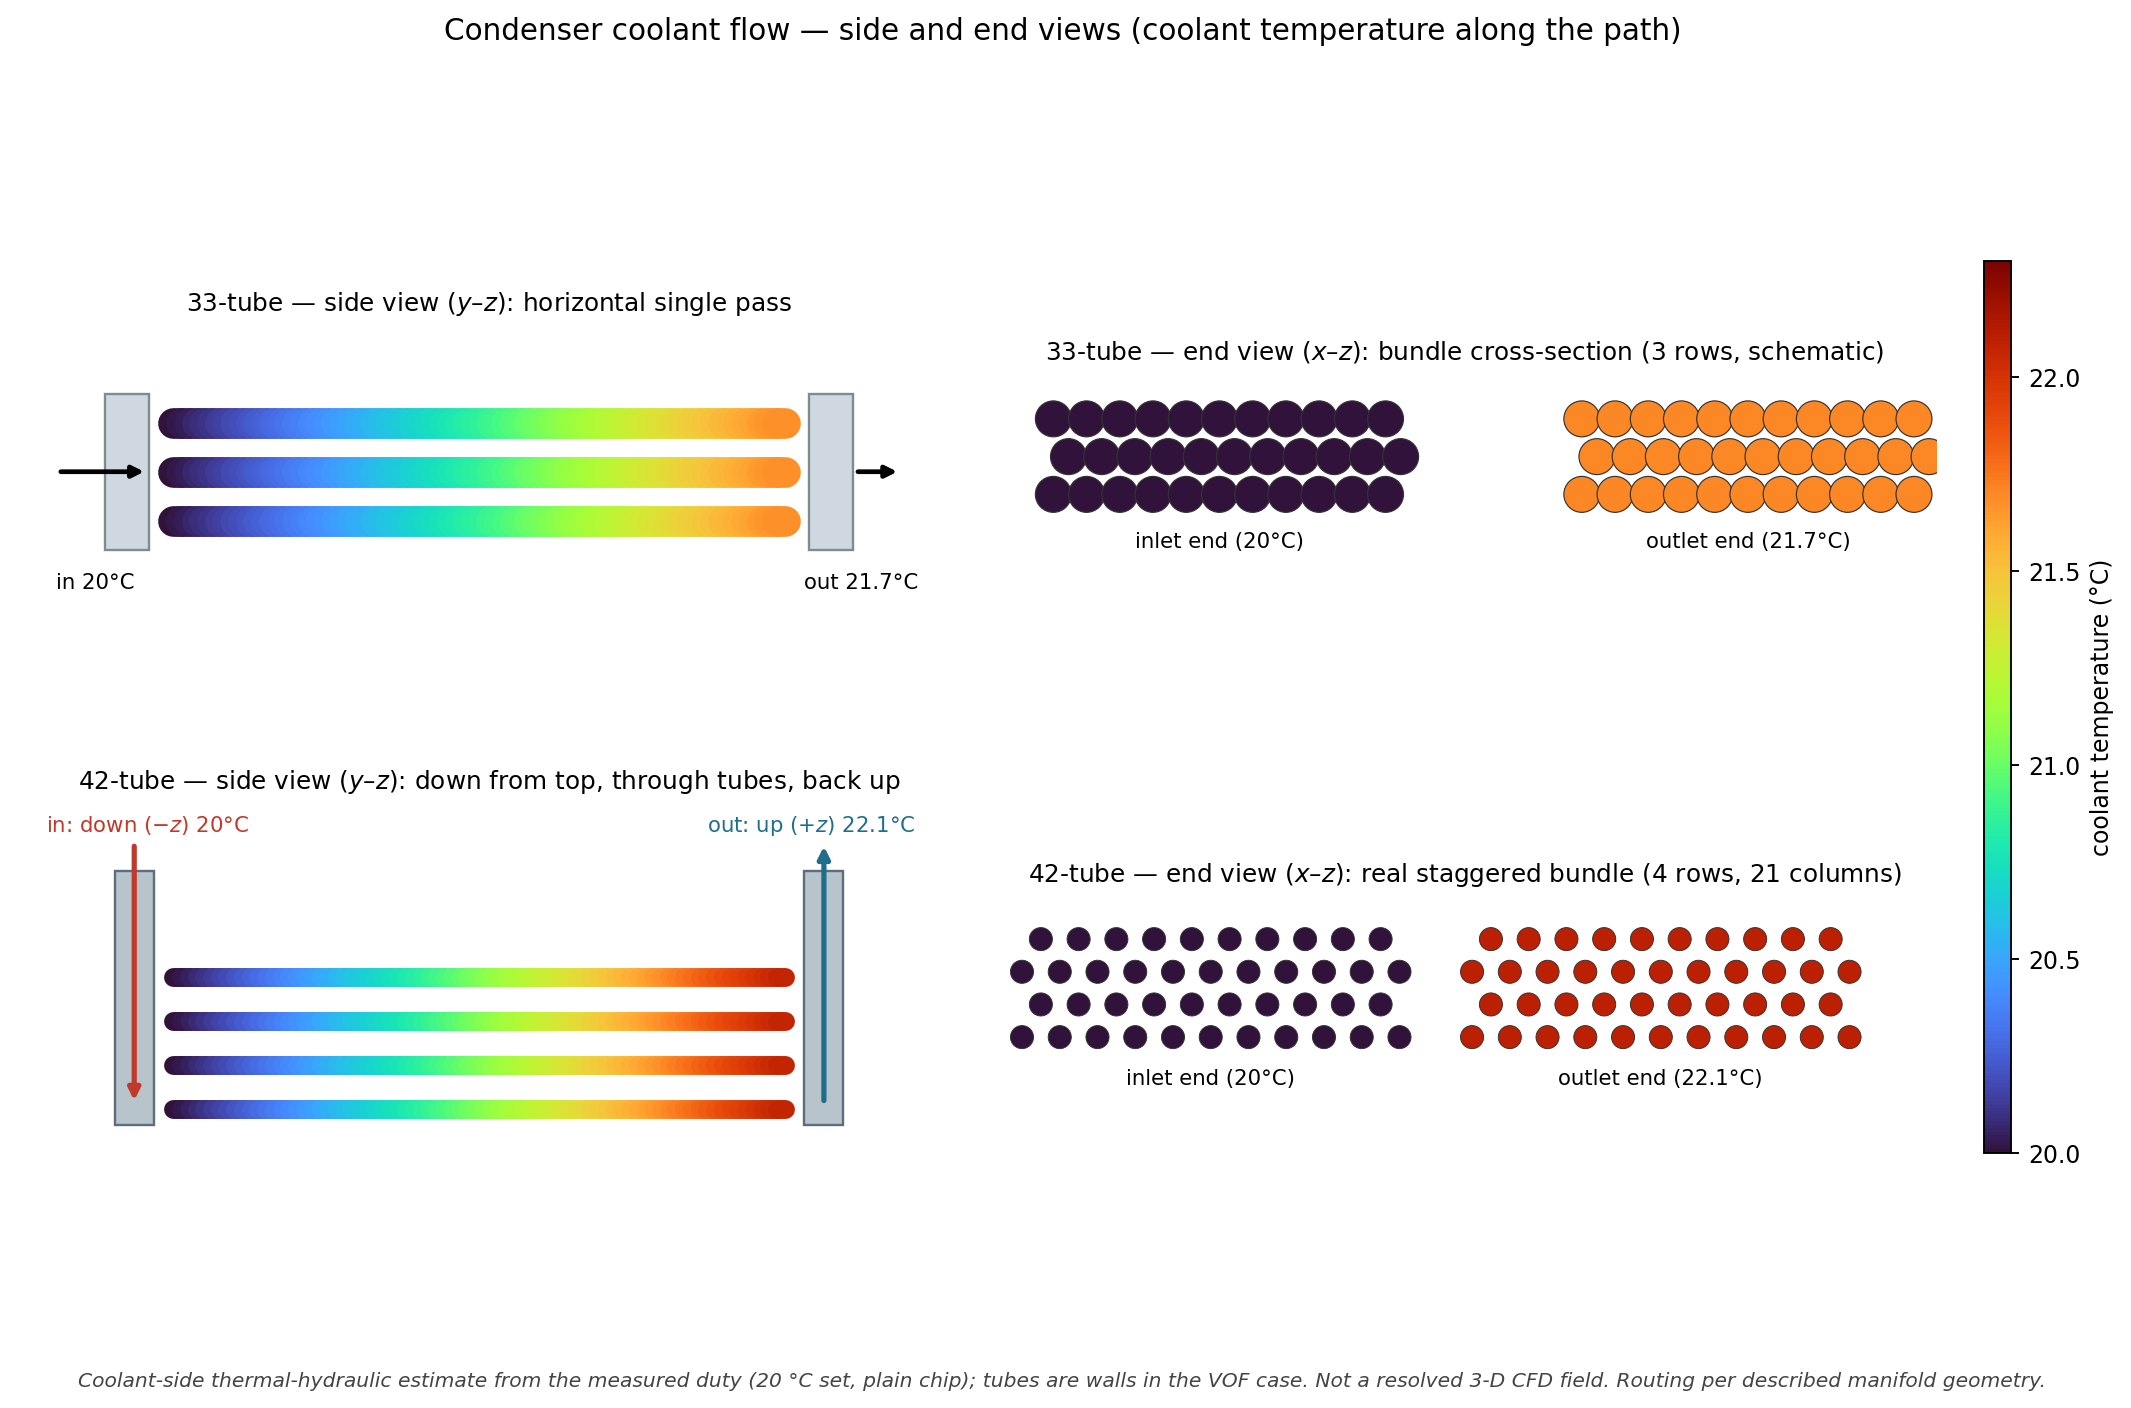
\includegraphics[width=0.98\textwidth]{fig_coolant_sideend.png}
\caption{Side ($y$--$z$) and end ($x$--$z$) views of the coolant path. Left: the 33-tube
horizontal single pass and the 42-tube down-from-top / through-tubes / back-up routing.
Right: bundle cross-sections at the inlet and outlet ends, with the real staggered 42-tube
layout. \emph{Coolant-side thermal-hydraulic estimate; not a resolved CFD field.}}
\label{of-fig:coolside}
\end{figure}

\section{Post-processing, diagnostics, and field contours}
\label{of-sec:post}
The case is analyzed with a PyVista post-processor that reads the OpenFOAM time
directories through the same reader ParaView uses (Fig.~\ref{of-fig:pipe}). Two data streams
are processed: the instantaneous fields, for interface dynamics and snapshots, and the
\texttt{fieldAverage} (time-averaged) fields, for the stationary quantities that are
compared with data. Geometry and the interface are drawn from the mesh patches and the
$\alpha=0.5$ isosurface.

\begin{figure}[H]
\centering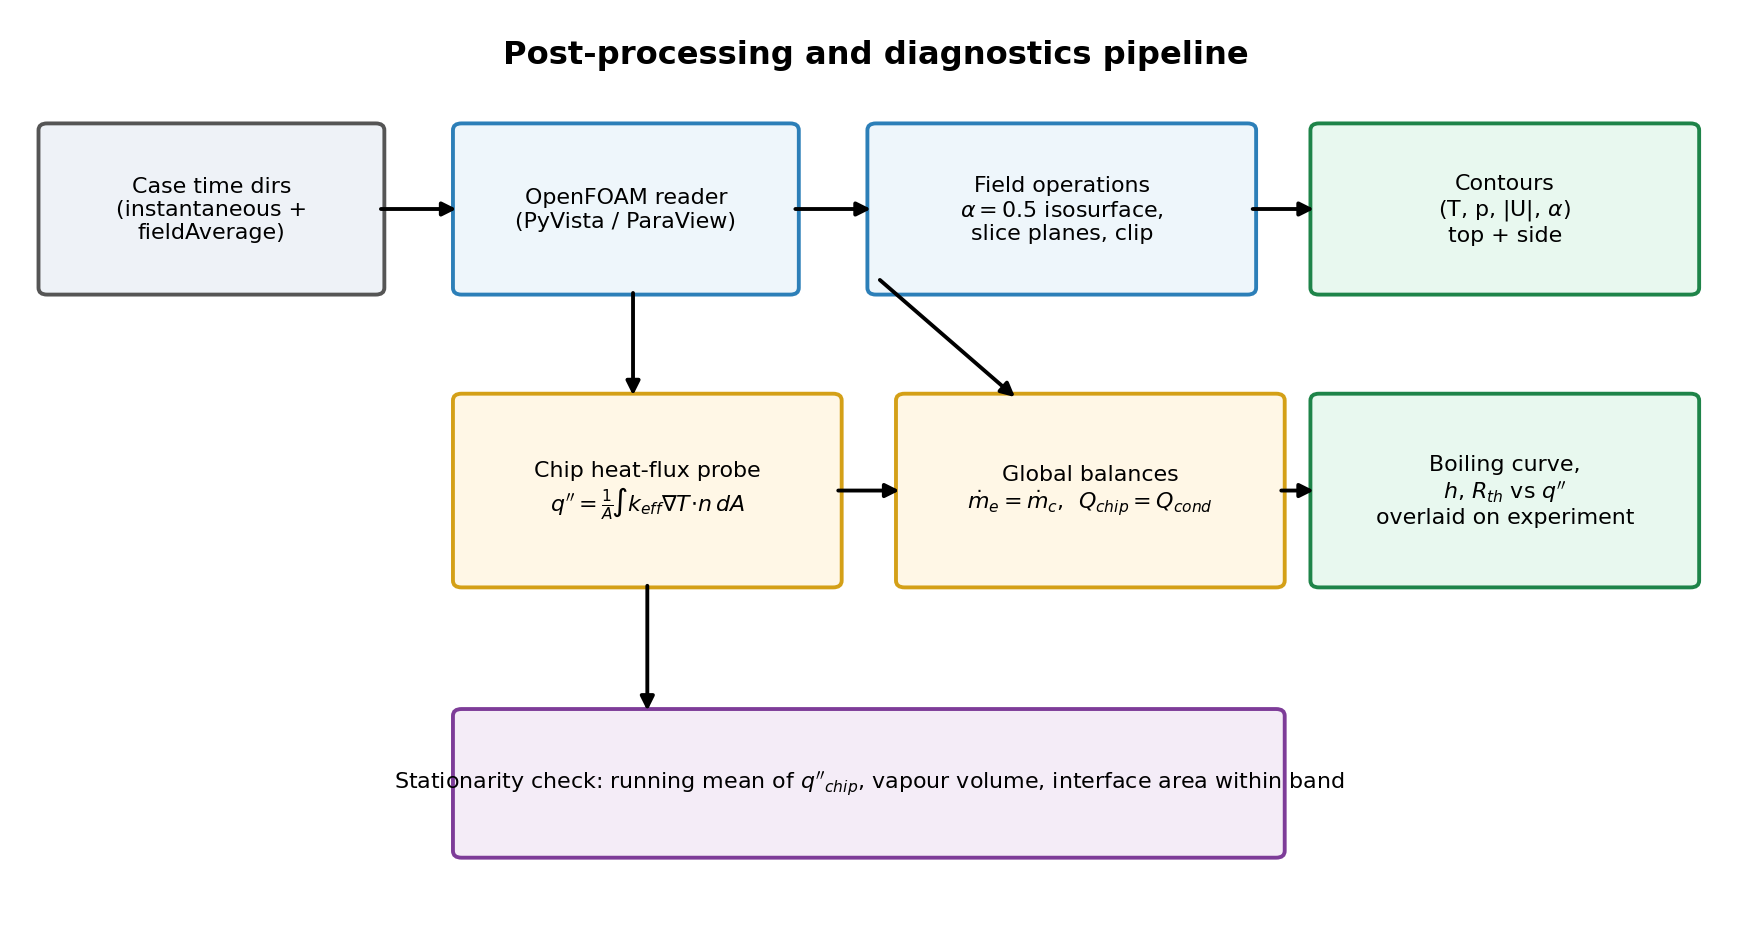
\includegraphics[width=0.95\textwidth]{fig_pipeline.png}
\caption{Post-processing and diagnostics pipeline, from the case time directories to
contours, global balances, and the boiling curve / resistance overlaid on experiment.}
\label{of-fig:pipe}
\end{figure}

\subsection{Chip heat-flux probe and the simulated boiling curve}
\label{of-sec:probe}
The simulated heat flux is the phase-weighted conductive flux integrated over the chip
patch and normalized by its area,
\begin{equation}
q''_{chip}=\frac{1}{A_{chip}}\int_{A_{chip}} k_{\mathrm{eff}}\,\nabla T\!\cdot\!\mathbf n
\,\mathrm dA,
\qquad k_{\mathrm{eff}}=\alpha k_l+(1-\alpha)k_v,
\label{of-eq:probe}
\end{equation}
evaluated on the time-averaged field. Sweeping the chip wall temperature and recording the
stationary $q''_{chip}$ traces out the simulated boiling curve, which is the quantity
fitted to the measured curve during calibration and overlaid on Fig.~\ref{of-fig:boil} for
validation. The boiling heat-transfer coefficient and the simulated thermal resistance
follow directly,
\begin{equation}
h=\frac{q''_{chip}}{T_{surf}-T_{sat}},\qquad
R_{tot}^{\mathrm{CFD}}=\frac{T_{surf}-T_{in}}{q''_{chip}A_{chip}},
\end{equation}
the latter compared against the measured and reduced-order values of Table~\ref{of-tab:res}.

\subsection{Global balances and verification}
At statistical stationarity the chamber must close two balances (Fig.~\ref{of-fig:bal}),
which serve as solver-level verification independent of any experimental comparison: net
evaporation equals net condensation, and the chip heat input equals the condenser heat
removal, both carried by the latent flux,
\begin{equation}
\int_V \dot m_e\,\mathrm dV=\int_V \dot m_c\,\mathrm dV,
\qquad
Q_{chip}=Q_{cond}=h_{fg}\!\int_V \dot m_e\,\mathrm dV .
\end{equation}
The condenser side is cross-checked against the measured coolant calorimetry of
Table~\ref{of-tab:coolant}, $Q_{cond}=\dot m_{cool}c_p(T_{out}-T_{in})$; a converged run that
violates these balances beyond a small tolerance is rejected regardless of how well a
single field matches.

\begin{figure}[H]
\centering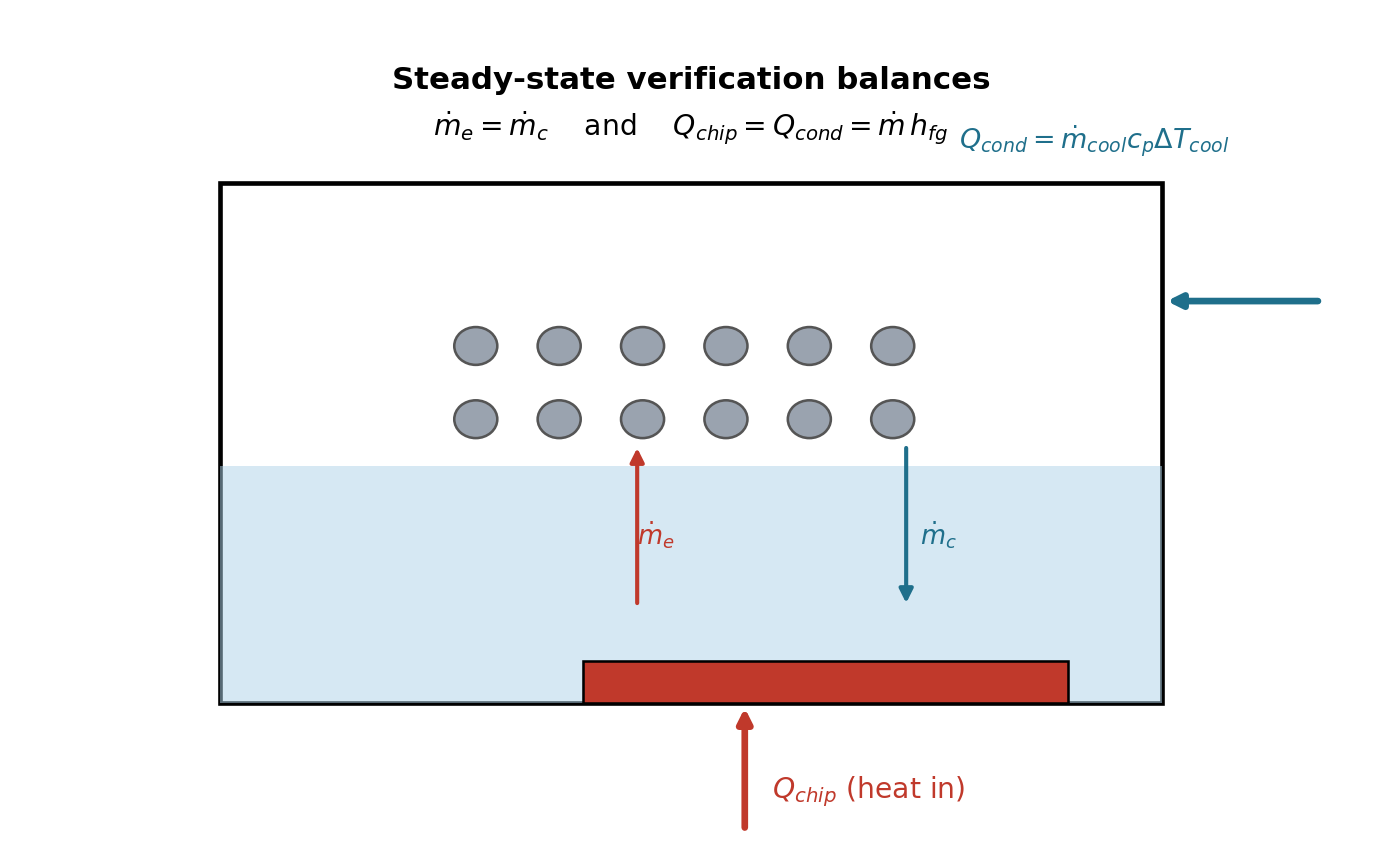
\includegraphics[width=0.62\textwidth]{fig_balance.png}
\caption{Steady-state verification balances: evaporation at the chip equals condensation at
the tubes, and the chip heat input equals the condenser duty set by the measured coolant
temperature rise.}
\label{of-fig:bal}
\end{figure}

\subsection{Stationarity, convergence, and mesh sensitivity}
A boiling simulation never reaches a steady state pointwise; the diagnostics are declared
converged when the running means of three integral monitors, the chip heat flux
$q''_{chip}$, the total vapor volume $\int(1-\alpha)\,\mathrm dV$, and the interfacial area
$\int|\nabla\alpha|\,\mathrm dV$, settle within a fixed band over a sliding window, with
their time averages no longer drifting. Mesh sensitivity is then established by repeating
the converged run on the mesh levels of Table~\ref{of-tab:mesh} and reporting the grid
convergence index (GCI) on $q''_{chip}$ and CHF; the production grid is selected where the
GCI falls below the measurement-uncertainty band (Section~\ref{of-sec:next}, item~1).

\subsection{Sampling planes, lines, and derived fields}
Scalar fields are extracted on two planes and two lines (Fig.~\ref{of-fig:planes}): a
horizontal $x$--$y$ plane through the bundle (\emph{top view}) and the vertical $x$--$z$
mid-plane (\emph{side view}) for contours, a vertical line above the chip center for
temperature and velocity profiles through the thermal boundary layer and interface, and a
horizontal midline through the bundle for the tube-to-tube field variation. From these,
the derived fields reported are the heat-transfer coefficient, the interfacial area density
$|\nabla\alpha|$, and the local vapor generation rate $\dot m_e$. The plane locations and
the color treatment are fixed here so the contour figures populate unchanged once the
converged run is available.

\begin{figure}[H]
\centering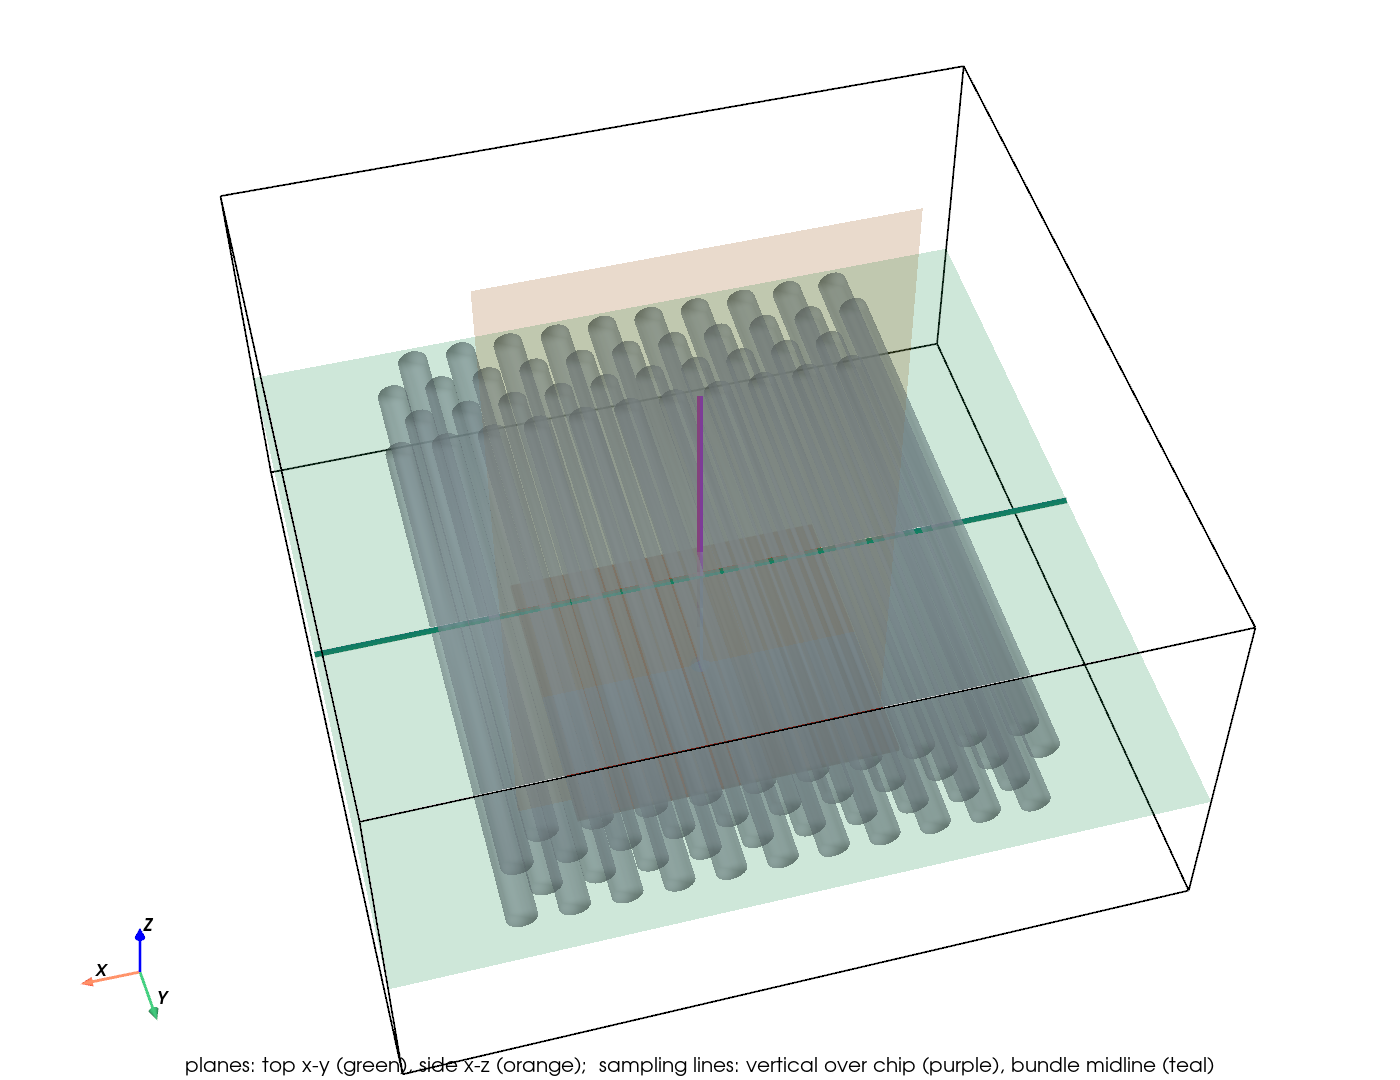
\includegraphics[width=0.62\textwidth]{fig_sampling.png}
\caption{Sampling geometry: top-view ($x$--$y$, green) and side-view ($x$--$z$, orange)
contour planes, with a vertical profile line above the chip (purple) and the bundle midline
(teal).}
\label{of-fig:planes}
\end{figure}

\subsection{Verification and single-phase reference fields}
Before any phase-change field is trusted, the setup is checked against two fields that are
known independently of the VOF solution (Fig.~\ref{of-fig:ref}). The hydrostatic pressure
$p=\rho_l g\,(z_{fill}-z)$ in the pool is analytic and is the rest-state limit the
$p_{rgh}$ solution must recover with $\mathbf U\to 0$. The single-phase conduction field,
$\nabla\!\cdot(k\nabla T)=0$ with the chip and tubes held at their wall temperatures and
the outer walls adiabatic, is solved here on the real $x$--$z$ geometry and bounds the
thermal field in the no-flow, no-boiling limit; it localizes the conductive resistance
around the chip and the cold sink at the tubes. \textbf{These are verification references,
not the VOF phase-change result}, boiling and convection make the actual pool far more
uniform and concentrate the gradients into thin interfacial layers. They confirm the
boundary-condition setup and provide a conduction-only bound; they do not predict the
boiling fields.

\begin{figure}[H]
\centering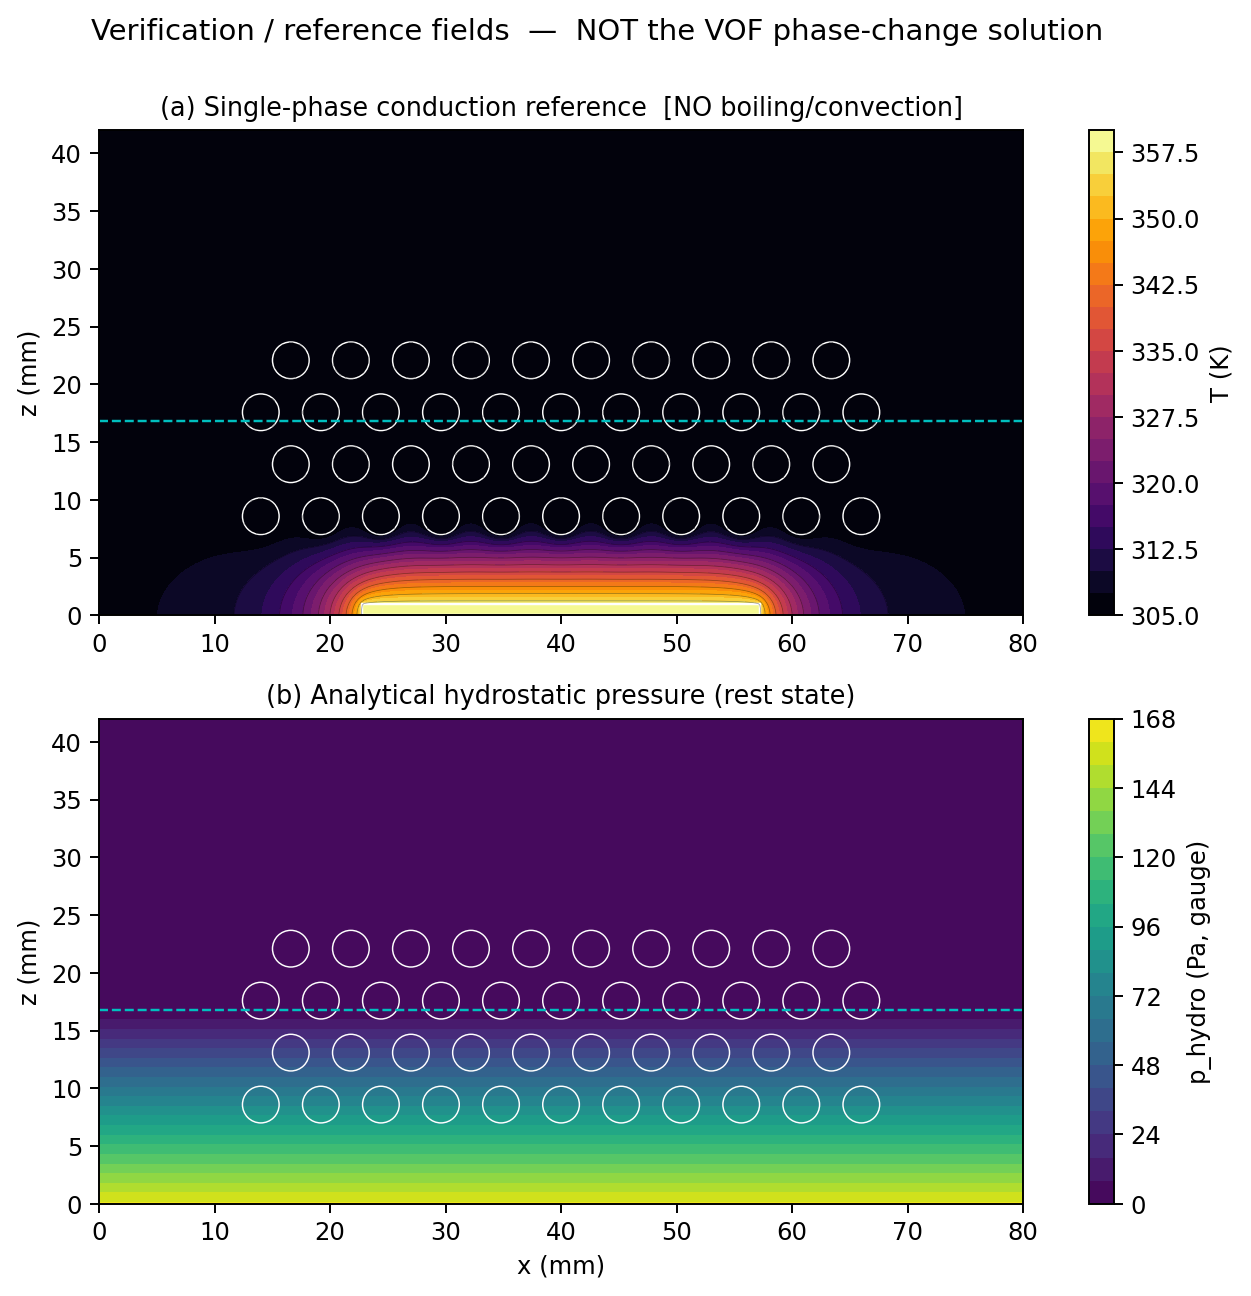
\includegraphics[width=0.82\textwidth]{fig_reffields.png}
\caption{Verification / reference fields on the $x$--$z$ plane: (a) single-phase steady
conduction with the chip and tubes at their wall temperatures (no boiling or convection);
(b) analytical hydrostatic pressure. \textbf{Neither is the VOF phase-change solution};
they verify the boundary-condition setup and bound the no-flow limit.}
\label{of-fig:ref}
\end{figure}

\subsection{Field contours (pending the converged run)}
The following are produced by the production run (Section~\ref{of-sec:reference} workflow) and
are intentionally left as reserved slots; no surrogate or unconverged fields are shown as
results:
\begin{itemize}
\item \emph{Temperature contours}, top ($x$--$y$) and side ($x$--$z$) views, for the
42-tube and 33-tube bundles.
\item \emph{Pressure contours}, top and side views, for both bundles.
\item \emph{Velocity-magnitude} and interface ($\alpha$) fields on the same planes, with the
profiles along the sampling lines of Fig.~\ref{of-fig:planes}.
\item \emph{CFD-to-experiment overlay}: the simulated boiling curve and thermal resistance
from the time-averaged probe, Eq.~\eqref{of-eq:probe}, overlaid on Figs.~\ref{of-fig:boil} and
\ref{of-fig:res} for both condensers, with the CHF turn-over checked against the measured
value.
\end{itemize}
The demonstration temperature and velocity fields carry non-physical extremes and are
clamped for display only; they are not presented as results.

\section{A reduced-cost two-dimensional demonstration}
\label{of-sec:twod}
The three-dimensional case in the preceding sections resolves the real bundle at production
mesh resolution and is correspondingly expensive to run to a stationary state. To exercise the
same phase-change pipeline at low cost, the project also includes a two-dimensional cross-section
case (\texttt{openfoam/chamber42\_2d}). It is a deliberate simplification with a clearly bounded
purpose: exercise the same phase-change pipeline cheaply and establish what such a reduced model
can and cannot deliver.

The two-dimensional mesh is generated by \texttt{blockMesh} alone, one cell thick in the
out-of-plane direction with empty front and back patches. The chip is a native floor patch,
obtained by splitting the streamwise direction into three blocks (left floor, chip, right
floor) rather than by feature extraction, so no \texttt{snappyHexMesh}, surface mesh, or
patch surgery is required and the mesh is fully reproducible. The condenser is idealised as
the cold top surface at the bundle-top height, held at the coolant temperature; resolving the
forty-two circular tubes in two dimensions would require \texttt{snappyHexMesh}, whose
isotropic refinement subdivides the single out-of-plane cell and breaks the empty-patch
two-dimensional constraint. The resolved tube bundle therefore remains the three-dimensional
domain, and the two-dimensional case carries the condenser only as a cold boundary. The
operating point is set to the measured 42-tube, plain-chip, \SI{20}{\celsius}-coolant
condition, with saturation \SI{322}{\kelvin} and the cold surface at \SI{293}{\kelvin}.

The intended calibration method is the chip heat-flux probe of Section~\ref{of-sec:probe} driving
a Nelder--Mead search over the evaporation and condensation rate coefficients: the chip wall
temperature is swept across the measured range and the time-averaged chip flux is matched to the
measured curve, with the evaporation coefficient the primary boiling-branch knob. Running this
case on a single workstation core under ESI OpenFOAM~v2512 establishes three things about that
method, each of which bears directly on the production run.

First, the pipeline is sound end to end. The \texttt{blockMesh} mesh passes \texttt{checkMesh},
the solver reads the phase-change model and advances stably with the temperature field bounded
between the coolant and chip values, and the coded probe compiles at run time and records the
chip heat flux. The machinery built for the three-dimensional case runs unmodified on the
two-dimensional surrogate.

Second, driven beyond the measured critical heat flux the model reproduces the boiling crisis.
With the chip held \SI{36}{\kelvin} above saturation, past the measured
\SI{65}{\watt\per\centi\meter\squared} CHF, vapour accumulates at the surface, coalesces into a
film after roughly \SI{60}{\milli\second}, and the chip heat flux collapses toward zero as the
low-conductivity vapour blankets the wall. This dryout is the one regime in which the phase
change visibly governs the surface flux.

Third, and decisively for the calibration strategy, on the nucleate branch the chip flux is
conduction-dominated and essentially independent of the Lee coefficient at this mesh resolution.
Holding the wall at \SI{65}{\celsius} (\SI{16}{\kelvin} superheat) and tripling the evaporation
coefficient from \num{0.1} to \num{0.3} leaves the chip heat flux unchanged to four significant
figures and the domain vapour fraction unchanged in the sixth decimal place
(Table~\ref{of-tab:2dsens}). The subcooled pool and the absence of resolved nucleation sites mean
that only a thin near-wall band of cells ever exceeds saturation, so the integrated evaporation
source is negligible and the surface flux is set by transient conduction into the slowly warming
pool rather than by boiling. That bulk warm-up is a seconds-scale diffusion process across the
\SI{24}{\milli\meter} gap, so at the sub-second times affordable on a single core the chip flux
has not stationarised, and no value of the rate coefficient changes that.

\begin{table}[ht]
\centering
\caption{Chip heat flux at a \SI{65}{\celsius} wall (\SI{16}{\kelvin} superheat), fixed
\SI{0.1}{\second} solve. Tripling the Lee evaporation coefficient leaves both the surface flux
and the domain vapour inventory essentially unchanged: at this two-dimensional mesh resolution
the phase-change source has no leverage on the measured quantity.}
\label{of-tab:2dsens}
\begin{tabular}{lcc}
\toprule
Lee evaporation coeff.\ $C_e$ & Chip flux $q''$ (\si{\watt\per\centi\meter\squared}) & Domain liquid fraction \\
\midrule
0.1 & 10.30 & 0.7385951 \\
0.3 & 10.30 & 0.7385937 \\
\bottomrule
\end{tabular}
\end{table}

\begin{figure}[ht]
\centering
\begin{subfigure}{0.49\textwidth}
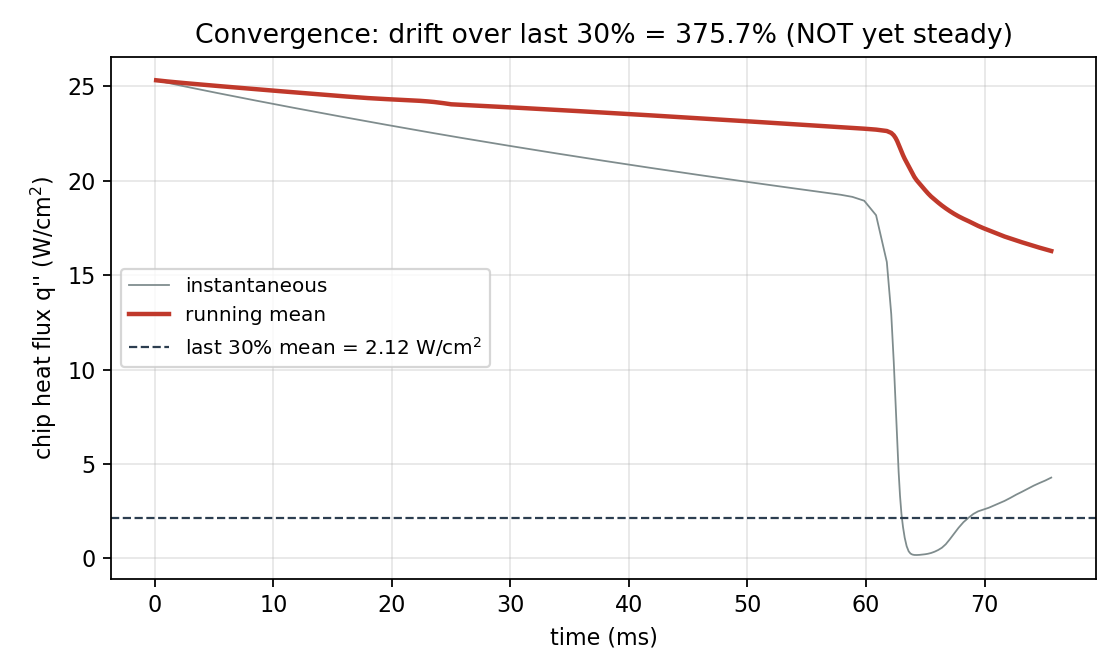
\includegraphics[width=\linewidth]{twod_nucleate}
\caption{Nucleate point (\SI{65}{\celsius} wall, \SI{16}{\kelvin} superheat): the chip flux
decays monotonically and has not stationarised at \SI{0.1}{\second}.}
\end{subfigure}\hfill
\begin{subfigure}{0.49\textwidth}
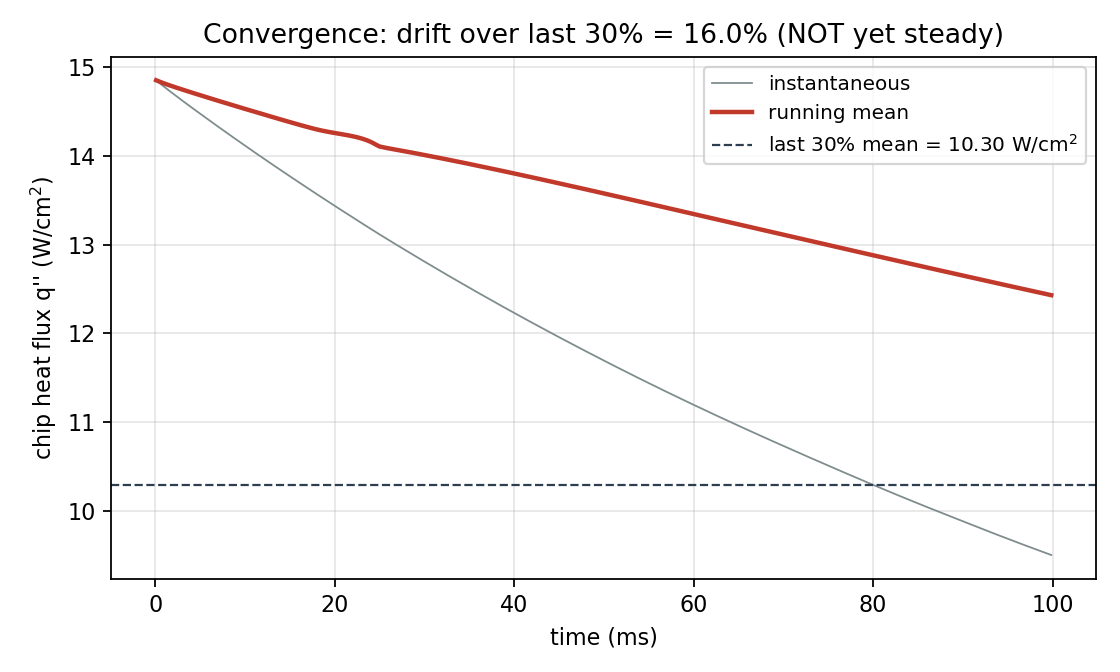
\includegraphics[width=\linewidth]{twod_collapse}
\caption{Past CHF (\SI{85}{\celsius} wall, \SI{36}{\kelvin} superheat): a vapour film forms near
\SI{63}{\milli\second} and the chip flux collapses toward zero (boiling crisis).}
\end{subfigure}
\caption{Two-dimensional demonstration runs on a single core under ESI OpenFOAM~v2512. The
nucleate branch is conduction-dominated and slow to settle; driven past the measured CHF the
model exhibits vapour-film dryout. Both traces are early-transient and non-converged, consistent
with the Lee-coefficient insensitivity of Table~\ref{of-tab:2dsens}.}
\label{of-fig:twod}
\end{figure}

The consequence is that the quantitative calibration cannot be performed on the two-dimensional
surrogate (Figure~\ref{of-fig:twod}): the coefficient the calibration must fit has no leverage on the quantity it is fitted
against, because the mesh does not resolve the boiling. This is a statement about resolution, not cost
alone. The resolved-bubble, snapped-and-layered three-dimensional mesh described above is not
merely a finer, slower computation; it is the resolution at which the Lee source becomes a
dominant term in the surface energy balance and the calibration becomes well-posed. The two-dimensional case is therefore a validated demonstration that the pipeline
runs and behaves physically at its limits, and direct evidence for where the quantitative work
must be done, not a substitute for it.

\section{Next steps}
\label{of-sec:next}
\begin{enumerate}
\item \textbf{Overlay the measurement-uncertainty bands} on the reference boiling-curve and
resistance figures (Figs.~\ref{of-fig:boil}, \ref{of-fig:res}). The propagated bands (heat flux
\SIrange{4}{11}{\%}, CHF $\sim\pm\SI{4}{\%}$), quantified in the companion reduced-order study,
define the tolerance against which any CFD-to-experiment agreement is judged.
\item \textbf{Refine and run the 42-tube case} at production resolution: snapped/layered mesh at
\SIrange{0.1}{0.3}{mm}, calibrate $C_E$/$C_C$ against the 42-tube/plain boiling curve and
CHF, and run to a statistically stationary state.
\item \textbf{Produce the field contours} (temperature, pressure, velocity, interface) on
the top and side planes of Fig.~\ref{of-fig:planes} and insert them in Section~\ref{of-sec:post}.
\item \textbf{Build and run the 33-tube CFD case} (open-manifold geometry) so the
cross-condenser comparison, larger/fewer tubes versus smaller/denser, is resolved in 3D and
not only in the reduced-order model.
\item \textbf{Resolve the coolant side} with a separate internal-flow or conjugate
heat-transfer simulation of each manifold and tube bundle, replacing the fixed-temperature
wall with a computed tube-wall temperature and capturing coolant velocity, pressure drop, and
header maldistribution; the thermal-hydraulic estimate of Section~\ref{of-sec:coolant} is the
one-dimensional limit of this.
\item \textbf{Overlay the converged CFD on experiment} for both condensers
(Figs.~\ref{of-fig:boil}, \ref{of-fig:res}) and report the CFD thermal resistance against
Table~\ref{of-tab:res}; passing requires lying within the uncertainty band point by point.
\item \textbf{Add the microchannel surface} to the CFD, either resolved or as a calibrated
sub-grid enhancement, and validate against the microchannel boiling curves.
\item \textbf{Verify the CHF mechanism in the converged solution}, checking whether the
simulation reproduces the heat-flux turnover and vapor-blanket dryout anticipated by the
two-dimensional demonstration (Section~\ref{of-sec:twod}); the experimental burnout-versus-ceiling
determination is carried out in the companion reduced-order study.
\item \textbf{Extend to the 66-tube bundle and HFE-7000} once those datasets are available,
to test cross-geometry and cross-fluid generalization in 3D.
\end{enumerate}

\section{Status and outlook}
\label{of-sec:status}
This document establishes a reproducible 3D VOF phase-change framework on the true
geometry: a verified body-fitted meshing pipeline (\num{299656} cells, \texttt{checkMesh}
OK), a complete physics, geometry, and numerics specification, the measured condenser
coolant operating conditions, and the full set of experimental and reduced-order
validation targets, boiling curves and thermal resistances for both condensers. What
remains is the computational campaign of Section~\ref{of-sec:next}: calibration, the run to stationarity,
the field contours, and the CFD-to-experiment overlay, together with the independent
prerequisite of quantifying the uncertainty band. On completion, the framework yields
resolved boiling and condensation fields that complement, and stress-test, the validated
reduced-order model of the same apparatus.

\clearpage
\begin{thebibliography}{9}
\small
\bibitem{shukla2024} Shukla, M.~Y., and Kandlikar, S.~G., 2024, ``Novel subcooled boiling chamber with submerged condensation for high heat flux removal for data center application,'' \textit{Proc.\ 23rd IEEE Intersociety Conf.\ on Thermal and Thermomechanical Phenomena in Electronic Systems (ITherm)}, Orlando, FL.
\bibitem{of-weller1998} Weller, H.~G., Tabor, G., Jasak, H., and Fureby, C., 1998, ``A
tensorial approach to computational continuum mechanics using object-oriented
techniques,'' \textit{Comput.\ Phys.}, 12(6), pp.~620--631.
\bibitem{of-hirt1981} Hirt, C.~W., and Nichols, B.~D., 1981, ``Volume of fluid (VOF) method
for the dynamics of free boundaries,'' \textit{J.\ Comput.\ Phys.}, 39(1), pp.~201--225.
\bibitem{of-brackbill1992} Brackbill, J.~U., Kothe, D.~B., and Zemach, C., 1992, ``A continuum
method for modeling surface tension,'' \textit{J.\ Comput.\ Phys.}, 100(2), pp.~335--354.
\bibitem{of-lee1980} Lee, W.~H., 1980, ``A pressure iteration scheme for two-phase flow
modeling,'' in \textit{Multiphase Transport}, Hemisphere.
\end{thebibliography}

\end{document}
